\input{config.tex}
\usepackage{array,tikz}
\newcolumntype{C}[1]{>{\centering\arraybackslash}p{#1}}
\graphicspath{{imagenes/tema10/}}
\title{Interpolación II}
\subtitle{Matemáticas 2}
\author{Grado en Ingeniería Informática}
\date{}
\begin{document}
\begin{frame}[t]{Interpolación II}
\titlepage
\end{frame}
\begin{frame}[t]{Interpolación de Hermite}
En algunos problemas conocemos los valores de una función y también los de sus derivadas.
\bigskip
Por ejemplo, en cinemática: posición, velocidad y aceleración.
\bigskip
La interpolación de Hermite incorpora los valores de $f'(x)$, además de los de $f(x)$, en la construcción del polinomio.
\end{frame}
\begin{frame}[t]{Hermite: expresión}
\small Para $n+1$ nodos distintos, el interpolante de Hermite tiene grado $\le2n+1$:
\[H_{2n+1}(x)=\sum_{i=0}^n f(x_i)h_{n,i}(x)+\sum_{i=0}^n f'(x_i)\widehat h_{n,i}(x),\]
donde
\[h_{n,i}(x)=\big[1-2(x-x_i)L'_{n,i}(x_i)\big]L_{n,i}(x)^2,\]
\[\widehat h_{n,i}(x)=(x-x_i)L_{n,i}(x)^2.\]
$L_{n,i}$ es el correspondiente multiplicador de Lagrange.
\end{frame}
\begin{frame}[t]{Hermite: número de condiciones}
Para $n+1$ puntos se utilizan:
\begin{itemize}
\item $n+1$ valores de $f(x)$.
\item $n+1$ valores de $f'(x)$.
\end{itemize}
\[H_{2n+1}(x_i)=f(x_i),\qquad H'_{2n+1}(x_i)=f'(x_i).\]
El grado máximo es $2n+1$, que es impar. El grado efectivo puede ser menor.
\end{frame}
\begin{frame}[t]{Hermite: error}
\small Si $f$ tiene $2n+2$ derivadas continuas en un intervalo que contiene los nodos y el punto $x$, entonces
\[f(x)-H_{2n+1}(x)=\frac{f^{(2n+2)}(\xi)}{(2n+2)!}\prod_{i=0}^n(x-x_i)^2,\]
para algún $\xi$ en el intervalo comprendido entre $x$ y los nodos.
\[\xi\in\big[\min\{x,x_0,\ldots,x_n\},\ \max\{x,x_0,\ldots,x_n\}\big].\]
\end{frame}
\begin{frame}[t]{Hermite mediante tablas}
La interpolación de Hermite también puede calcularse mediante una adaptación del método de diferencias divididas.
\bigskip
En esta versión, cada nodo aparece dos veces y los valores de las derivadas resuelven las diferencias divididas de nodos repetidos.
\end{frame}
\begin{frame}[t]{Recordatorio: diferencias divididas}
\par\noindent\begin{minipage}[t][13mm][t]{\textwidth}\small\strut Diferencias divididas para nodos distintos.\end{minipage}\par\nointerlineskip
\begin{center}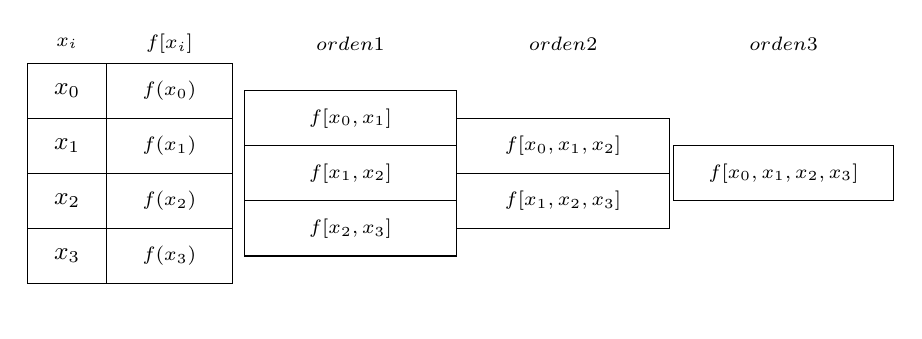
\begin{tikzpicture}[x=1cm,y=1cm]\path[use as bounding box] (0,-3.6) rectangle (11,0);
\node[font=\scriptsize] at (0.5,-.2) {$x_i$};
\node[font=\scriptsize] at (1.8,-.2) {$f[x_i]$};
\node[font=\scriptsize] at (4.1,-.2) {$\text{orden }1$};
\node[font=\scriptsize] at (6.8,-.2) {$\text{orden }2$};
\node[font=\scriptsize] at (9.6,-.2) {$\text{orden }3$};
\node[draw,minimum width=1cm,minimum height=.7cm,font=\small] at (.5,-0.8) {$x_0$};
\node[draw,minimum width=1cm,minimum height=.7cm,font=\small] at (.5,-1.5) {$x_1$};
\node[draw,minimum width=1cm,minimum height=.7cm,font=\small] at (.5,-2.2) {$x_2$};
\node[draw,minimum width=1cm,minimum height=.7cm,font=\small] at (.5,-2.8999999999999995) {$x_3$};
\node[draw,minimum width=1.6cm,minimum height=.7cm,font=\scriptsize,inner sep=1pt] at (1.8,-0.8) {$f(x_0)$};
\node[draw,minimum width=1.6cm,minimum height=.7cm,font=\scriptsize,inner sep=1pt] at (1.8,-1.5) {$f(x_1)$};
\node[draw,minimum width=1.6cm,minimum height=.7cm,font=\scriptsize,inner sep=1pt] at (1.8,-2.2) {$f(x_2)$};
\node[draw,minimum width=1.6cm,minimum height=.7cm,font=\scriptsize,inner sep=1pt] at (1.8,-2.8999999999999995) {$f(x_3)$};
\node[draw,minimum width=2.7cm,minimum height=.7cm,font=\scriptsize,inner sep=1pt] at (4.1,-1.15) {$f[x_0,x_1]$};
\node[draw,minimum width=2.7cm,minimum height=.7cm,font=\scriptsize,inner sep=1pt] at (4.1,-1.85) {$f[x_1,x_2]$};
\node[draw,minimum width=2.7cm,minimum height=.7cm,font=\scriptsize,inner sep=1pt] at (4.1,-2.5500000000000003) {$f[x_2,x_3]$};
\node[draw,minimum width=2.7cm,minimum height=.7cm,font=\scriptsize,inner sep=1pt] at (6.8,-1.5) {$f[x_0,x_1,x_2]$};
\node[draw,minimum width=2.7cm,minimum height=.7cm,font=\scriptsize,inner sep=1pt] at (6.8,-2.2) {$f[x_1,x_2,x_3]$};
\node[draw,minimum width=2.8cm,minimum height=.7cm,font=\scriptsize,inner sep=1pt] at (9.6,-1.8499999999999999) {$f[x_0,x_1,x_2,x_3]$};
\end{tikzpicture}\end{center}\small\[f[x_i]=f(x_i).\]\[f[x_i,x_{i+1}]=\frac{f(x_{i+1})-f(x_i)}{x_{i+1}-x_i}.\]
\end{frame}
\begin{frame}[t]{Hermite: nodos repetidos}
\scriptsize
\[H_{2n+1}(x)=f[z_0]+\sum_{k=1}^{2n+1}f[z_0,\ldots,z_k]\prod_{j=0}^{k-1}(x-z_j).\]
Para $i=0,\ldots,n$:
\[z_{2i}=z_{2i+1}=x_i,\qquad f[z_{2i}]=f[z_{2i+1}]=f(x_i),\]
\[f[z_{2i},z_{2i+1}]=f'(x_i).\]
Entre dos nodos distintos se calcula la diferencia dividida habitual:
\[f[z_{2i-1},z_{2i}]=\frac{f[z_{2i}]-f[z_{2i-1}]}{z_{2i}-z_{2i-1}},\quad i=1,\ldots,n.\]
Para órdenes $k\ge2$ se usa la recurrencia ordinaria:
\[f[z_i,\ldots,z_{i+k}]=\frac{f[z_{i+1},\ldots,z_{i+k}]-f[z_i,\ldots,z_{i+k-1}]}{z_{i+k}-z_i}.\]
\end{frame}
\begin{frame}[t]{Hermite: tabla de diferencias}
\par\noindent\begin{minipage}[t][13mm][t]{\textwidth}\small\strut Cada nodo y su valor se repiten dos veces.\end{minipage}\par\nointerlineskip
\begin{center}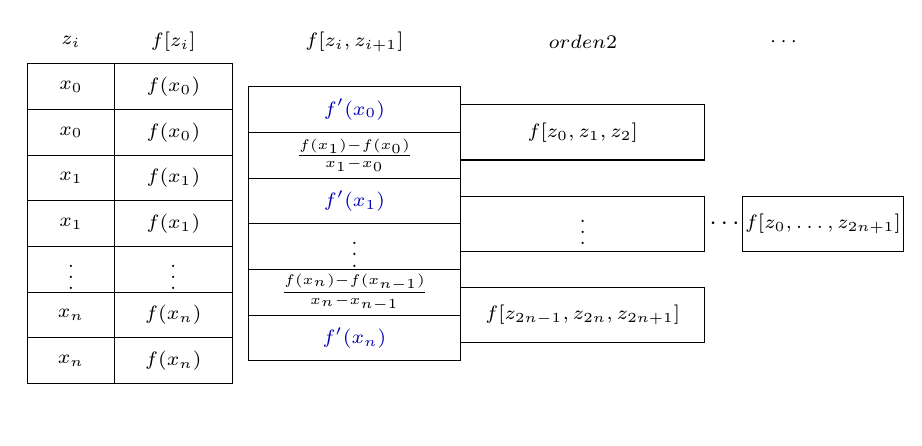
\begin{tikzpicture}[x=1cm,y=1cm]\path[use as bounding box] (0,-4.95) rectangle (11,0);
\node[font=\scriptsize] at (0.55,-.18) {$z_i$};
\node[font=\scriptsize] at (1.85,-.18) {$f[z_i]$};
\node[font=\scriptsize] at (4.15,-.18) {$f[z_i,z_{i+1}]$};
\node[font=\scriptsize] at (7.05,-.18) {$\text{orden }2$};
\node[font=\scriptsize] at (9.6,-.18) {$\cdots$};
\node[draw,minimum width=1.1cm,minimum height=.58cm,font=\scriptsize,inner sep=1pt] at (0.55,-0.75) {$x_0$};
\node[draw,minimum width=1.5cm,minimum height=.58cm,font=\scriptsize,inner sep=1pt] at (1.85,-0.75) {$f(x_0)$};
\node[draw,minimum width=1.1cm,minimum height=.58cm,font=\scriptsize,inner sep=1pt] at (0.55,-1.33) {$x_0$};
\node[draw,minimum width=1.5cm,minimum height=.58cm,font=\scriptsize,inner sep=1pt] at (1.85,-1.33) {$f(x_0)$};
\node[draw,minimum width=1.1cm,minimum height=.58cm,font=\scriptsize,inner sep=1pt] at (0.55,-1.91) {$x_1$};
\node[draw,minimum width=1.5cm,minimum height=.58cm,font=\scriptsize,inner sep=1pt] at (1.85,-1.91) {$f(x_1)$};
\node[draw,minimum width=1.1cm,minimum height=.58cm,font=\scriptsize,inner sep=1pt] at (0.55,-2.4899999999999998) {$x_1$};
\node[draw,minimum width=1.5cm,minimum height=.58cm,font=\scriptsize,inner sep=1pt] at (1.85,-2.4899999999999998) {$f(x_1)$};
\node[draw,minimum width=1.1cm,minimum height=.58cm,font=\scriptsize,inner sep=1pt] at (0.55,-3.07) {$\vdots$};
\node[draw,minimum width=1.5cm,minimum height=.58cm,font=\scriptsize,inner sep=1pt] at (1.85,-3.07) {$\vdots$};
\node[draw,minimum width=1.1cm,minimum height=.58cm,font=\scriptsize,inner sep=1pt] at (0.55,-3.65) {$x_n$};
\node[draw,minimum width=1.5cm,minimum height=.58cm,font=\scriptsize,inner sep=1pt] at (1.85,-3.65) {$f(x_n)$};
\node[draw,minimum width=1.1cm,minimum height=.58cm,font=\scriptsize,inner sep=1pt] at (0.55,-4.2299999999999995) {$x_n$};
\node[draw,minimum width=1.5cm,minimum height=.58cm,font=\scriptsize,inner sep=1pt] at (1.85,-4.2299999999999995) {$f(x_n)$};
\node[draw,minimum width=2.7cm,minimum height=.58cm,font=\scriptsize,inner sep=1pt,text=blue!70!black] at (4.15,-1.04) {$f'(x_0)$};
\node[draw,minimum width=2.7cm,minimum height=.58cm,font=\scriptsize,inner sep=1pt] at (4.15,-1.62) {$\frac{f(x_1)-f(x_0)}{x_1-x_0}$};
\node[draw,minimum width=2.7cm,minimum height=.58cm,font=\scriptsize,inner sep=1pt,text=blue!70!black] at (4.15,-2.1999999999999997) {$f'(x_1)$};
\node[draw,minimum width=2.7cm,minimum height=.58cm,font=\scriptsize,inner sep=1pt] at (4.15,-2.78) {$\vdots$};
\node[draw,minimum width=2.7cm,minimum height=.58cm,font=\scriptsize,inner sep=1pt] at (4.15,-3.36) {$\frac{f(x_n)-f(x_{n-1})}{x_n-x_{n-1}}$};
\node[draw,minimum width=2.7cm,minimum height=.58cm,font=\scriptsize,inner sep=1pt,text=blue!70!black] at (4.15,-3.94) {$f'(x_n)$};
\node[draw,minimum width=3.1cm,minimum height=.7cm,font=\scriptsize,inner sep=1pt] at (7.05,-1.33) {$f[z_0,z_1,z_2]$};
\node[draw,minimum width=3.1cm,minimum height=.7cm,font=\scriptsize,inner sep=1pt] at (7.05,-2.49) {$\vdots$};
\node[draw,minimum width=3.1cm,minimum height=.7cm,font=\scriptsize,inner sep=1pt] at (7.05,-3.65) {$f[z_{2n-1},z_{2n},z_{2n+1}]$};
\node[font=\small] at (8.85,-2.49) {$\cdots$};\node[draw,minimum width=1.6cm,minimum height=.7cm,font=\scriptsize,inner sep=1pt] at (10.1,-2.49) {$f[z_0,\ldots,z_{2n+1}]$};\end{tikzpicture}\end{center}
\end{frame}
\begin{frame}[t]{Derivadas en la tabla de Hermite}
\small
Las dos primeras columnas, $z_i$ y $f[z_i]$, contienen nodos y valores duplicados.
\medskip
La primera columna de diferencias intercala los valores $f'(x_i)$ con los cocientes habituales.
\[\frac{f(x_i)-f(x_i)}{x_i-x_i}=\frac00\]
se sustituye por $f[x_i,x_i]=f'(x_i)$.
\medskip
Desde la segunda diferencia dividida, la tabla se calcula con la recurrencia ordinaria.
\end{frame}
\begin{frame}[t]{Hermite: diferencias de primer orden}
\par\noindent\begin{minipage}[t][13mm][t]{\textwidth}\small\strut Los valores de las derivadas ocupan las diferencias entre nodos repetidos.\end{minipage}\par\nointerlineskip
\begin{center}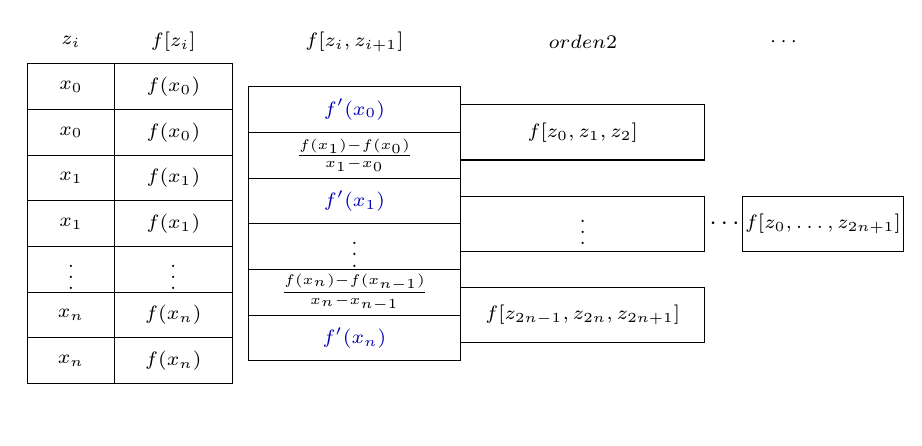
\begin{tikzpicture}[x=1cm,y=1cm]\path[use as bounding box] (0,-4.95) rectangle (11,0);
\node[font=\scriptsize] at (0.55,-.18) {$z_i$};
\node[font=\scriptsize] at (1.85,-.18) {$f[z_i]$};
\node[font=\scriptsize] at (4.15,-.18) {$f[z_i,z_{i+1}]$};
\node[font=\scriptsize] at (7.05,-.18) {$\text{orden }2$};
\node[font=\scriptsize] at (9.6,-.18) {$\cdots$};
\node[draw,minimum width=1.1cm,minimum height=.58cm,font=\scriptsize,inner sep=1pt] at (0.55,-0.75) {$x_0$};
\node[draw,minimum width=1.5cm,minimum height=.58cm,font=\scriptsize,inner sep=1pt] at (1.85,-0.75) {$f(x_0)$};
\node[draw,minimum width=1.1cm,minimum height=.58cm,font=\scriptsize,inner sep=1pt] at (0.55,-1.33) {$x_0$};
\node[draw,minimum width=1.5cm,minimum height=.58cm,font=\scriptsize,inner sep=1pt] at (1.85,-1.33) {$f(x_0)$};
\node[draw,minimum width=1.1cm,minimum height=.58cm,font=\scriptsize,inner sep=1pt] at (0.55,-1.91) {$x_1$};
\node[draw,minimum width=1.5cm,minimum height=.58cm,font=\scriptsize,inner sep=1pt] at (1.85,-1.91) {$f(x_1)$};
\node[draw,minimum width=1.1cm,minimum height=.58cm,font=\scriptsize,inner sep=1pt] at (0.55,-2.4899999999999998) {$x_1$};
\node[draw,minimum width=1.5cm,minimum height=.58cm,font=\scriptsize,inner sep=1pt] at (1.85,-2.4899999999999998) {$f(x_1)$};
\node[draw,minimum width=1.1cm,minimum height=.58cm,font=\scriptsize,inner sep=1pt] at (0.55,-3.07) {$\vdots$};
\node[draw,minimum width=1.5cm,minimum height=.58cm,font=\scriptsize,inner sep=1pt] at (1.85,-3.07) {$\vdots$};
\node[draw,minimum width=1.1cm,minimum height=.58cm,font=\scriptsize,inner sep=1pt] at (0.55,-3.65) {$x_n$};
\node[draw,minimum width=1.5cm,minimum height=.58cm,font=\scriptsize,inner sep=1pt] at (1.85,-3.65) {$f(x_n)$};
\node[draw,minimum width=1.1cm,minimum height=.58cm,font=\scriptsize,inner sep=1pt] at (0.55,-4.2299999999999995) {$x_n$};
\node[draw,minimum width=1.5cm,minimum height=.58cm,font=\scriptsize,inner sep=1pt] at (1.85,-4.2299999999999995) {$f(x_n)$};
\node[draw,minimum width=2.7cm,minimum height=.58cm,font=\scriptsize,inner sep=1pt,text=blue!70!black] at (4.15,-1.04) {$f'(x_0)$};
\node[draw,minimum width=2.7cm,minimum height=.58cm,font=\scriptsize,inner sep=1pt] at (4.15,-1.62) {$\frac{f(x_1)-f(x_0)}{x_1-x_0}$};
\node[draw,minimum width=2.7cm,minimum height=.58cm,font=\scriptsize,inner sep=1pt,text=blue!70!black] at (4.15,-2.1999999999999997) {$f'(x_1)$};
\node[draw,minimum width=2.7cm,minimum height=.58cm,font=\scriptsize,inner sep=1pt] at (4.15,-2.78) {$\vdots$};
\node[draw,minimum width=2.7cm,minimum height=.58cm,font=\scriptsize,inner sep=1pt] at (4.15,-3.36) {$\frac{f(x_n)-f(x_{n-1})}{x_n-x_{n-1}}$};
\node[draw,minimum width=2.7cm,minimum height=.58cm,font=\scriptsize,inner sep=1pt,text=blue!70!black] at (4.15,-3.94) {$f'(x_n)$};
\node[draw,minimum width=3.1cm,minimum height=.7cm,font=\scriptsize,inner sep=1pt] at (7.05,-1.33) {$f[z_0,z_1,z_2]$};
\node[draw,minimum width=3.1cm,minimum height=.7cm,font=\scriptsize,inner sep=1pt] at (7.05,-2.49) {$\vdots$};
\node[draw,minimum width=3.1cm,minimum height=.7cm,font=\scriptsize,inner sep=1pt] at (7.05,-3.65) {$f[z_{2n-1},z_{2n},z_{2n+1}]$};
\node[font=\small] at (8.85,-2.49) {$\cdots$};\node[draw,minimum width=1.6cm,minimum height=.7cm,font=\scriptsize,inner sep=1pt] at (10.1,-2.49) {$f[z_0,\ldots,z_{2n+1}]$};\end{tikzpicture}\end{center}
\end{frame}
\begin{frame}[t]{Hermite: diferencias de orden superior}
\par\noindent\begin{minipage}[t][13mm][t]{\textwidth}\small\strut Las columnas siguientes se calculan con la recurrencia habitual.\end{minipage}\par\nointerlineskip
\begin{center}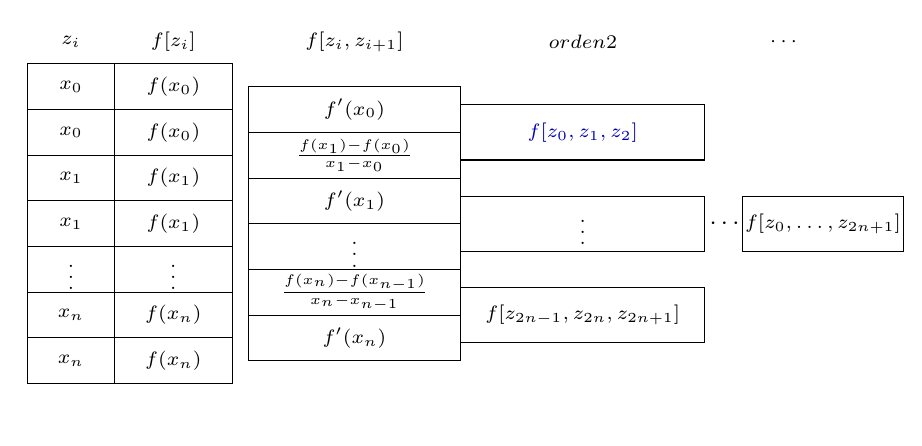
\begin{tikzpicture}[x=1cm,y=1cm]\path[use as bounding box] (0,-4.95) rectangle (11,0);
\node[font=\scriptsize] at (0.55,-.18) {$z_i$};
\node[font=\scriptsize] at (1.85,-.18) {$f[z_i]$};
\node[font=\scriptsize] at (4.15,-.18) {$f[z_i,z_{i+1}]$};
\node[font=\scriptsize] at (7.05,-.18) {$\text{orden }2$};
\node[font=\scriptsize] at (9.6,-.18) {$\cdots$};
\node[draw,minimum width=1.1cm,minimum height=.58cm,font=\scriptsize,inner sep=1pt] at (0.55,-0.75) {$x_0$};
\node[draw,minimum width=1.5cm,minimum height=.58cm,font=\scriptsize,inner sep=1pt] at (1.85,-0.75) {$f(x_0)$};
\node[draw,minimum width=1.1cm,minimum height=.58cm,font=\scriptsize,inner sep=1pt] at (0.55,-1.33) {$x_0$};
\node[draw,minimum width=1.5cm,minimum height=.58cm,font=\scriptsize,inner sep=1pt] at (1.85,-1.33) {$f(x_0)$};
\node[draw,minimum width=1.1cm,minimum height=.58cm,font=\scriptsize,inner sep=1pt] at (0.55,-1.91) {$x_1$};
\node[draw,minimum width=1.5cm,minimum height=.58cm,font=\scriptsize,inner sep=1pt] at (1.85,-1.91) {$f(x_1)$};
\node[draw,minimum width=1.1cm,minimum height=.58cm,font=\scriptsize,inner sep=1pt] at (0.55,-2.4899999999999998) {$x_1$};
\node[draw,minimum width=1.5cm,minimum height=.58cm,font=\scriptsize,inner sep=1pt] at (1.85,-2.4899999999999998) {$f(x_1)$};
\node[draw,minimum width=1.1cm,minimum height=.58cm,font=\scriptsize,inner sep=1pt] at (0.55,-3.07) {$\vdots$};
\node[draw,minimum width=1.5cm,minimum height=.58cm,font=\scriptsize,inner sep=1pt] at (1.85,-3.07) {$\vdots$};
\node[draw,minimum width=1.1cm,minimum height=.58cm,font=\scriptsize,inner sep=1pt] at (0.55,-3.65) {$x_n$};
\node[draw,minimum width=1.5cm,minimum height=.58cm,font=\scriptsize,inner sep=1pt] at (1.85,-3.65) {$f(x_n)$};
\node[draw,minimum width=1.1cm,minimum height=.58cm,font=\scriptsize,inner sep=1pt] at (0.55,-4.2299999999999995) {$x_n$};
\node[draw,minimum width=1.5cm,minimum height=.58cm,font=\scriptsize,inner sep=1pt] at (1.85,-4.2299999999999995) {$f(x_n)$};
\node[draw,minimum width=2.7cm,minimum height=.58cm,font=\scriptsize,inner sep=1pt] at (4.15,-1.04) {$f'(x_0)$};
\node[draw,minimum width=2.7cm,minimum height=.58cm,font=\scriptsize,inner sep=1pt] at (4.15,-1.62) {$\frac{f(x_1)-f(x_0)}{x_1-x_0}$};
\node[draw,minimum width=2.7cm,minimum height=.58cm,font=\scriptsize,inner sep=1pt] at (4.15,-2.1999999999999997) {$f'(x_1)$};
\node[draw,minimum width=2.7cm,minimum height=.58cm,font=\scriptsize,inner sep=1pt] at (4.15,-2.78) {$\vdots$};
\node[draw,minimum width=2.7cm,minimum height=.58cm,font=\scriptsize,inner sep=1pt] at (4.15,-3.36) {$\frac{f(x_n)-f(x_{n-1})}{x_n-x_{n-1}}$};
\node[draw,minimum width=2.7cm,minimum height=.58cm,font=\scriptsize,inner sep=1pt] at (4.15,-3.94) {$f'(x_n)$};
\node[draw,minimum width=3.1cm,minimum height=.7cm,font=\scriptsize,inner sep=1pt,text=blue!70!black] at (7.05,-1.33) {$f[z_0,z_1,z_2]$};
\node[draw,minimum width=3.1cm,minimum height=.7cm,font=\scriptsize,inner sep=1pt] at (7.05,-2.49) {$\vdots$};
\node[draw,minimum width=3.1cm,minimum height=.7cm,font=\scriptsize,inner sep=1pt] at (7.05,-3.65) {$f[z_{2n-1},z_{2n},z_{2n+1}]$};
\node[font=\small] at (8.85,-2.49) {$\cdots$};\node[draw,minimum width=1.6cm,minimum height=.7cm,font=\scriptsize,inner sep=1pt] at (10.1,-2.49) {$f[z_0,\ldots,z_{2n+1}]$};\end{tikzpicture}\end{center}
\end{frame}
\begin{frame}[t]{Hermite: ejemplo}
\par\noindent\begin{minipage}[t][13mm][t]{\textwidth}\small\strut $f(x)=(x/2)^{x-2}$, $f\prime(x)=f(x)\big((x-2)/x+\ln(x/2)\big)$.\end{minipage}\par\nointerlineskip
\begin{minipage}[t]{\textwidth}\begin{center}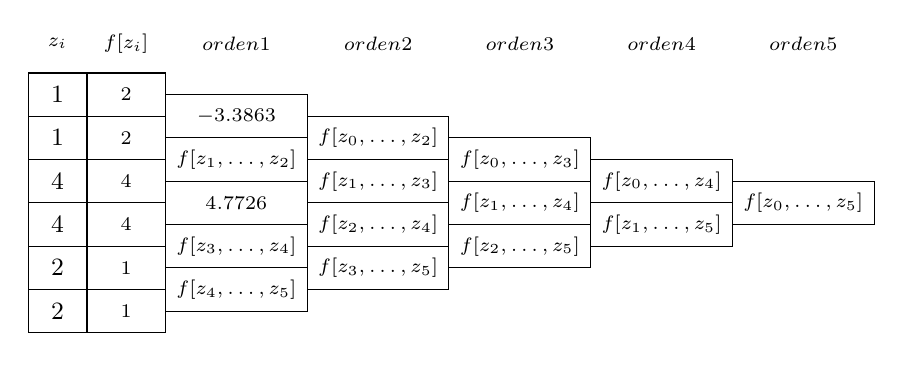
\begin{tikzpicture}[x=1cm,y=1cm]\path[use as bounding box] (0,-4.10) rectangle (11,0);
\node[font=\scriptsize] at (0.38,-.2) {$z_i$};
\node[font=\scriptsize] at (1.25,-.2) {$f[z_i]$};
\node[font=\scriptsize] at (2.65,-.2) {$\text{orden }1$};
\node[font=\scriptsize] at (4.45,-.2) {$\text{orden }2$};
\node[font=\scriptsize] at (6.25,-.2) {$\text{orden }3$};
\node[font=\scriptsize] at (8.05,-.2) {$\text{orden }4$};
\node[font=\scriptsize] at (9.85,-.2) {$\text{orden }5$};
\node[draw,minimum width=.75cm,minimum height=.55cm,font=\small,inner sep=1pt] at (.38,-0.85) {$1$};
\node[draw,minimum width=.75cm,minimum height=.55cm,font=\small,inner sep=1pt] at (.38,-1.4) {$1$};
\node[draw,minimum width=.75cm,minimum height=.55cm,font=\small,inner sep=1pt] at (.38,-1.9500000000000002) {$4$};
\node[draw,minimum width=.75cm,minimum height=.55cm,font=\small,inner sep=1pt] at (.38,-2.5) {$4$};
\node[draw,minimum width=.75cm,minimum height=.55cm,font=\small,inner sep=1pt] at (.38,-3.0500000000000003) {$2$};
\node[draw,minimum width=.75cm,minimum height=.55cm,font=\small,inner sep=1pt] at (.38,-3.6) {$2$};
\node[draw,minimum width=1cm,minimum height=.55cm,font=\scriptsize,inner sep=1pt] at (1.25,-0.85) {$2$};
\node[draw,minimum width=1cm,minimum height=.55cm,font=\scriptsize,inner sep=1pt] at (1.25,-1.4) {$2$};
\node[draw,minimum width=1cm,minimum height=.55cm,font=\scriptsize,inner sep=1pt] at (1.25,-1.9500000000000002) {$4$};
\node[draw,minimum width=1cm,minimum height=.55cm,font=\scriptsize,inner sep=1pt] at (1.25,-2.5) {$4$};
\node[draw,minimum width=1cm,minimum height=.55cm,font=\scriptsize,inner sep=1pt] at (1.25,-3.0500000000000003) {$1$};
\node[draw,minimum width=1cm,minimum height=.55cm,font=\scriptsize,inner sep=1pt] at (1.25,-3.6) {$1$};
\node[draw,minimum width=1.8cm,minimum height=.55cm,font=\scriptsize,inner sep=1pt] at (2.65,-1.125) {$-3.3863$};
\node[draw,minimum width=1.8cm,minimum height=.55cm,font=\scriptsize,inner sep=1pt] at (2.65,-1.6749999999999998) {$f[z_1,\ldots,z_2]$};
\node[draw,minimum width=1.8cm,minimum height=.55cm,font=\scriptsize,inner sep=1pt] at (2.65,-2.225) {$4.7726$};
\node[draw,minimum width=1.8cm,minimum height=.55cm,font=\scriptsize,inner sep=1pt] at (2.65,-2.775) {$f[z_3,\ldots,z_4]$};
\node[draw,minimum width=1.8cm,minimum height=.55cm,font=\scriptsize,inner sep=1pt] at (2.65,-3.325) {$f[z_4,\ldots,z_5]$};
\node[draw,minimum width=1.8cm,minimum height=.55cm,font=\scriptsize,inner sep=1pt] at (4.45,-1.4) {$f[z_0,\ldots,z_2]$};
\node[draw,minimum width=1.8cm,minimum height=.55cm,font=\scriptsize,inner sep=1pt] at (4.45,-1.95) {$f[z_1,\ldots,z_3]$};
\node[draw,minimum width=1.8cm,minimum height=.55cm,font=\scriptsize,inner sep=1pt] at (4.45,-2.5) {$f[z_2,\ldots,z_4]$};
\node[draw,minimum width=1.8cm,minimum height=.55cm,font=\scriptsize,inner sep=1pt] at (4.45,-3.05) {$f[z_3,\ldots,z_5]$};
\node[draw,minimum width=1.8cm,minimum height=.55cm,font=\scriptsize,inner sep=1pt] at (6.25,-1.675) {$f[z_0,\ldots,z_3]$};
\node[draw,minimum width=1.8cm,minimum height=.55cm,font=\scriptsize,inner sep=1pt] at (6.25,-2.225) {$f[z_1,\ldots,z_4]$};
\node[draw,minimum width=1.8cm,minimum height=.55cm,font=\scriptsize,inner sep=1pt] at (6.25,-2.7750000000000004) {$f[z_2,\ldots,z_5]$};
\node[draw,minimum width=1.8cm,minimum height=.55cm,font=\scriptsize,inner sep=1pt] at (8.05,-1.9500000000000002) {$f[z_0,\ldots,z_4]$};
\node[draw,minimum width=1.8cm,minimum height=.55cm,font=\scriptsize,inner sep=1pt] at (8.05,-2.5) {$f[z_1,\ldots,z_5]$};
\node[draw,minimum width=1.8cm,minimum height=.55cm,font=\scriptsize,inner sep=1pt] at (9.85,-2.225) {$f[z_0,\ldots,z_5]$};
\end{tikzpicture}\end{center}\end{minipage}\par\scriptsize Los nodos repetidos son $1,1,4,4,2,2$.
\end{frame}
\begin{frame}[t]{Hermite: ejemplo}
\par\noindent\begin{minipage}[t][13mm][t]{\textwidth}\small\strut $f(x)=(x/2)^{x-2}$, $f\prime(x)=f(x)\big((x-2)/x+\ln(x/2)\big)$.\end{minipage}\par\nointerlineskip
\begin{minipage}[t]{\textwidth}\begin{center}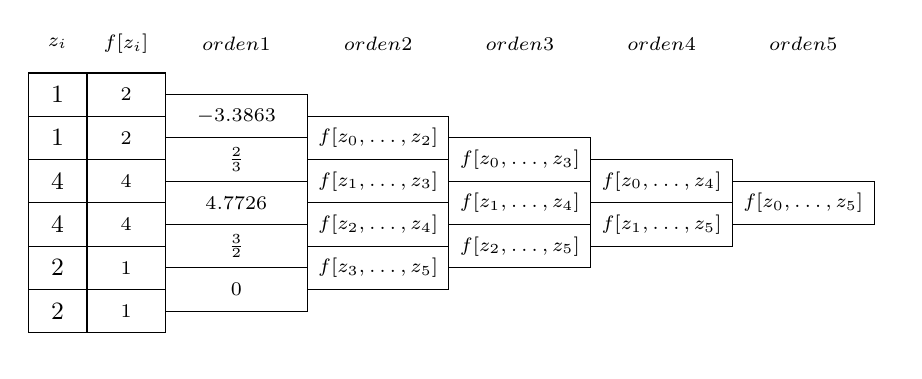
\begin{tikzpicture}[x=1cm,y=1cm]\path[use as bounding box] (0,-4.10) rectangle (11,0);
\node[font=\scriptsize] at (0.38,-.2) {$z_i$};
\node[font=\scriptsize] at (1.25,-.2) {$f[z_i]$};
\node[font=\scriptsize] at (2.65,-.2) {$\text{orden }1$};
\node[font=\scriptsize] at (4.45,-.2) {$\text{orden }2$};
\node[font=\scriptsize] at (6.25,-.2) {$\text{orden }3$};
\node[font=\scriptsize] at (8.05,-.2) {$\text{orden }4$};
\node[font=\scriptsize] at (9.85,-.2) {$\text{orden }5$};
\node[draw,minimum width=.75cm,minimum height=.55cm,font=\small,inner sep=1pt] at (.38,-0.85) {$1$};
\node[draw,minimum width=.75cm,minimum height=.55cm,font=\small,inner sep=1pt] at (.38,-1.4) {$1$};
\node[draw,minimum width=.75cm,minimum height=.55cm,font=\small,inner sep=1pt] at (.38,-1.9500000000000002) {$4$};
\node[draw,minimum width=.75cm,minimum height=.55cm,font=\small,inner sep=1pt] at (.38,-2.5) {$4$};
\node[draw,minimum width=.75cm,minimum height=.55cm,font=\small,inner sep=1pt] at (.38,-3.0500000000000003) {$2$};
\node[draw,minimum width=.75cm,minimum height=.55cm,font=\small,inner sep=1pt] at (.38,-3.6) {$2$};
\node[draw,minimum width=1cm,minimum height=.55cm,font=\scriptsize,inner sep=1pt] at (1.25,-0.85) {$2$};
\node[draw,minimum width=1cm,minimum height=.55cm,font=\scriptsize,inner sep=1pt] at (1.25,-1.4) {$2$};
\node[draw,minimum width=1cm,minimum height=.55cm,font=\scriptsize,inner sep=1pt] at (1.25,-1.9500000000000002) {$4$};
\node[draw,minimum width=1cm,minimum height=.55cm,font=\scriptsize,inner sep=1pt] at (1.25,-2.5) {$4$};
\node[draw,minimum width=1cm,minimum height=.55cm,font=\scriptsize,inner sep=1pt] at (1.25,-3.0500000000000003) {$1$};
\node[draw,minimum width=1cm,minimum height=.55cm,font=\scriptsize,inner sep=1pt] at (1.25,-3.6) {$1$};
\node[draw,minimum width=1.8cm,minimum height=.55cm,font=\scriptsize,inner sep=1pt] at (2.65,-1.125) {$-3.3863$};
\node[draw,minimum width=1.8cm,minimum height=.55cm,font=\scriptsize,inner sep=1pt] at (2.65,-1.6749999999999998) {$\frac23$};
\node[draw,minimum width=1.8cm,minimum height=.55cm,font=\scriptsize,inner sep=1pt] at (2.65,-2.225) {$4.7726$};
\node[draw,minimum width=1.8cm,minimum height=.55cm,font=\scriptsize,inner sep=1pt] at (2.65,-2.775) {$\frac32$};
\node[draw,minimum width=1.8cm,minimum height=.55cm,font=\scriptsize,inner sep=1pt] at (2.65,-3.325) {$0$};
\node[draw,minimum width=1.8cm,minimum height=.55cm,font=\scriptsize,inner sep=1pt] at (4.45,-1.4) {$f[z_0,\ldots,z_2]$};
\node[draw,minimum width=1.8cm,minimum height=.55cm,font=\scriptsize,inner sep=1pt] at (4.45,-1.95) {$f[z_1,\ldots,z_3]$};
\node[draw,minimum width=1.8cm,minimum height=.55cm,font=\scriptsize,inner sep=1pt] at (4.45,-2.5) {$f[z_2,\ldots,z_4]$};
\node[draw,minimum width=1.8cm,minimum height=.55cm,font=\scriptsize,inner sep=1pt] at (4.45,-3.05) {$f[z_3,\ldots,z_5]$};
\node[draw,minimum width=1.8cm,minimum height=.55cm,font=\scriptsize,inner sep=1pt] at (6.25,-1.675) {$f[z_0,\ldots,z_3]$};
\node[draw,minimum width=1.8cm,minimum height=.55cm,font=\scriptsize,inner sep=1pt] at (6.25,-2.225) {$f[z_1,\ldots,z_4]$};
\node[draw,minimum width=1.8cm,minimum height=.55cm,font=\scriptsize,inner sep=1pt] at (6.25,-2.7750000000000004) {$f[z_2,\ldots,z_5]$};
\node[draw,minimum width=1.8cm,minimum height=.55cm,font=\scriptsize,inner sep=1pt] at (8.05,-1.9500000000000002) {$f[z_0,\ldots,z_4]$};
\node[draw,minimum width=1.8cm,minimum height=.55cm,font=\scriptsize,inner sep=1pt] at (8.05,-2.5) {$f[z_1,\ldots,z_5]$};
\node[draw,minimum width=1.8cm,minimum height=.55cm,font=\scriptsize,inner sep=1pt] at (9.85,-2.225) {$f[z_0,\ldots,z_5]$};
\end{tikzpicture}\end{center}\end{minipage}\par\scriptsize Los nodos repetidos son $1,1,4,4,2,2$.
\end{frame}
\begin{frame}[t]{Hermite: ejemplo}
\par\noindent\begin{minipage}[t][13mm][t]{\textwidth}\small\strut $f(x)=(x/2)^{x-2}$, $f\prime(x)=f(x)\big((x-2)/x+\ln(x/2)\big)$.\end{minipage}\par\nointerlineskip
\begin{minipage}[t]{\textwidth}\begin{center}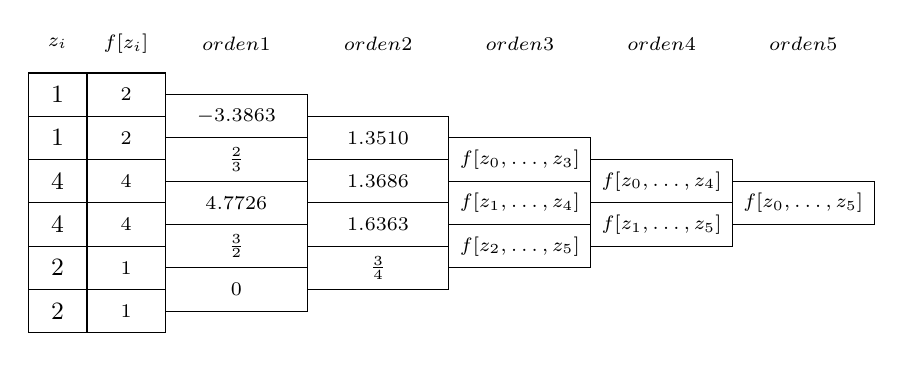
\begin{tikzpicture}[x=1cm,y=1cm]\path[use as bounding box] (0,-4.10) rectangle (11,0);
\node[font=\scriptsize] at (0.38,-.2) {$z_i$};
\node[font=\scriptsize] at (1.25,-.2) {$f[z_i]$};
\node[font=\scriptsize] at (2.65,-.2) {$\text{orden }1$};
\node[font=\scriptsize] at (4.45,-.2) {$\text{orden }2$};
\node[font=\scriptsize] at (6.25,-.2) {$\text{orden }3$};
\node[font=\scriptsize] at (8.05,-.2) {$\text{orden }4$};
\node[font=\scriptsize] at (9.85,-.2) {$\text{orden }5$};
\node[draw,minimum width=.75cm,minimum height=.55cm,font=\small,inner sep=1pt] at (.38,-0.85) {$1$};
\node[draw,minimum width=.75cm,minimum height=.55cm,font=\small,inner sep=1pt] at (.38,-1.4) {$1$};
\node[draw,minimum width=.75cm,minimum height=.55cm,font=\small,inner sep=1pt] at (.38,-1.9500000000000002) {$4$};
\node[draw,minimum width=.75cm,minimum height=.55cm,font=\small,inner sep=1pt] at (.38,-2.5) {$4$};
\node[draw,minimum width=.75cm,minimum height=.55cm,font=\small,inner sep=1pt] at (.38,-3.0500000000000003) {$2$};
\node[draw,minimum width=.75cm,minimum height=.55cm,font=\small,inner sep=1pt] at (.38,-3.6) {$2$};
\node[draw,minimum width=1cm,minimum height=.55cm,font=\scriptsize,inner sep=1pt] at (1.25,-0.85) {$2$};
\node[draw,minimum width=1cm,minimum height=.55cm,font=\scriptsize,inner sep=1pt] at (1.25,-1.4) {$2$};
\node[draw,minimum width=1cm,minimum height=.55cm,font=\scriptsize,inner sep=1pt] at (1.25,-1.9500000000000002) {$4$};
\node[draw,minimum width=1cm,minimum height=.55cm,font=\scriptsize,inner sep=1pt] at (1.25,-2.5) {$4$};
\node[draw,minimum width=1cm,minimum height=.55cm,font=\scriptsize,inner sep=1pt] at (1.25,-3.0500000000000003) {$1$};
\node[draw,minimum width=1cm,minimum height=.55cm,font=\scriptsize,inner sep=1pt] at (1.25,-3.6) {$1$};
\node[draw,minimum width=1.8cm,minimum height=.55cm,font=\scriptsize,inner sep=1pt] at (2.65,-1.125) {$-3.3863$};
\node[draw,minimum width=1.8cm,minimum height=.55cm,font=\scriptsize,inner sep=1pt] at (2.65,-1.6749999999999998) {$\frac23$};
\node[draw,minimum width=1.8cm,minimum height=.55cm,font=\scriptsize,inner sep=1pt] at (2.65,-2.225) {$4.7726$};
\node[draw,minimum width=1.8cm,minimum height=.55cm,font=\scriptsize,inner sep=1pt] at (2.65,-2.775) {$\frac32$};
\node[draw,minimum width=1.8cm,minimum height=.55cm,font=\scriptsize,inner sep=1pt] at (2.65,-3.325) {$0$};
\node[draw,minimum width=1.8cm,minimum height=.55cm,font=\scriptsize,inner sep=1pt] at (4.45,-1.4) {$1.3510$};
\node[draw,minimum width=1.8cm,minimum height=.55cm,font=\scriptsize,inner sep=1pt] at (4.45,-1.95) {$1.3686$};
\node[draw,minimum width=1.8cm,minimum height=.55cm,font=\scriptsize,inner sep=1pt] at (4.45,-2.5) {$1.6363$};
\node[draw,minimum width=1.8cm,minimum height=.55cm,font=\scriptsize,inner sep=1pt] at (4.45,-3.05) {$\frac34$};
\node[draw,minimum width=1.8cm,minimum height=.55cm,font=\scriptsize,inner sep=1pt] at (6.25,-1.675) {$f[z_0,\ldots,z_3]$};
\node[draw,minimum width=1.8cm,minimum height=.55cm,font=\scriptsize,inner sep=1pt] at (6.25,-2.225) {$f[z_1,\ldots,z_4]$};
\node[draw,minimum width=1.8cm,minimum height=.55cm,font=\scriptsize,inner sep=1pt] at (6.25,-2.7750000000000004) {$f[z_2,\ldots,z_5]$};
\node[draw,minimum width=1.8cm,minimum height=.55cm,font=\scriptsize,inner sep=1pt] at (8.05,-1.9500000000000002) {$f[z_0,\ldots,z_4]$};
\node[draw,minimum width=1.8cm,minimum height=.55cm,font=\scriptsize,inner sep=1pt] at (8.05,-2.5) {$f[z_1,\ldots,z_5]$};
\node[draw,minimum width=1.8cm,minimum height=.55cm,font=\scriptsize,inner sep=1pt] at (9.85,-2.225) {$f[z_0,\ldots,z_5]$};
\end{tikzpicture}\end{center}\end{minipage}\par\scriptsize Los nodos repetidos son $1,1,4,4,2,2$.
\end{frame}
\begin{frame}[t]{Hermite: ejemplo}
\par\noindent\begin{minipage}[t][13mm][t]{\textwidth}\small\strut $f(x)=(x/2)^{x-2}$, $f\prime(x)=f(x)\big((x-2)/x+\ln(x/2)\big)$.\end{minipage}\par\nointerlineskip
\begin{minipage}[t]{\textwidth}\begin{center}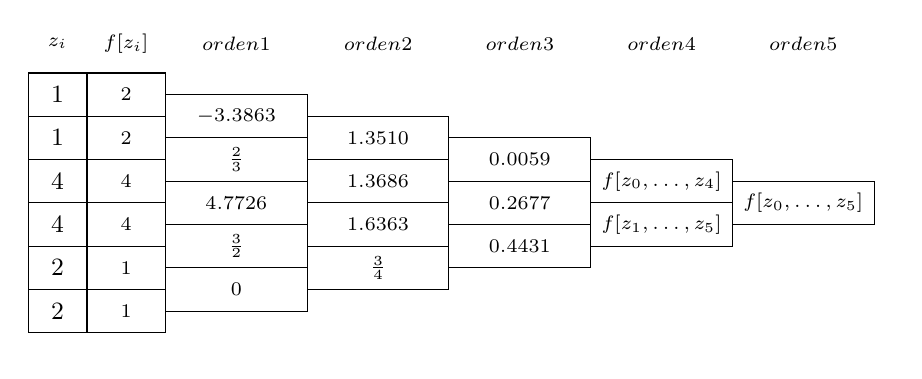
\begin{tikzpicture}[x=1cm,y=1cm]\path[use as bounding box] (0,-4.10) rectangle (11,0);
\node[font=\scriptsize] at (0.38,-.2) {$z_i$};
\node[font=\scriptsize] at (1.25,-.2) {$f[z_i]$};
\node[font=\scriptsize] at (2.65,-.2) {$\text{orden }1$};
\node[font=\scriptsize] at (4.45,-.2) {$\text{orden }2$};
\node[font=\scriptsize] at (6.25,-.2) {$\text{orden }3$};
\node[font=\scriptsize] at (8.05,-.2) {$\text{orden }4$};
\node[font=\scriptsize] at (9.85,-.2) {$\text{orden }5$};
\node[draw,minimum width=.75cm,minimum height=.55cm,font=\small,inner sep=1pt] at (.38,-0.85) {$1$};
\node[draw,minimum width=.75cm,minimum height=.55cm,font=\small,inner sep=1pt] at (.38,-1.4) {$1$};
\node[draw,minimum width=.75cm,minimum height=.55cm,font=\small,inner sep=1pt] at (.38,-1.9500000000000002) {$4$};
\node[draw,minimum width=.75cm,minimum height=.55cm,font=\small,inner sep=1pt] at (.38,-2.5) {$4$};
\node[draw,minimum width=.75cm,minimum height=.55cm,font=\small,inner sep=1pt] at (.38,-3.0500000000000003) {$2$};
\node[draw,minimum width=.75cm,minimum height=.55cm,font=\small,inner sep=1pt] at (.38,-3.6) {$2$};
\node[draw,minimum width=1cm,minimum height=.55cm,font=\scriptsize,inner sep=1pt] at (1.25,-0.85) {$2$};
\node[draw,minimum width=1cm,minimum height=.55cm,font=\scriptsize,inner sep=1pt] at (1.25,-1.4) {$2$};
\node[draw,minimum width=1cm,minimum height=.55cm,font=\scriptsize,inner sep=1pt] at (1.25,-1.9500000000000002) {$4$};
\node[draw,minimum width=1cm,minimum height=.55cm,font=\scriptsize,inner sep=1pt] at (1.25,-2.5) {$4$};
\node[draw,minimum width=1cm,minimum height=.55cm,font=\scriptsize,inner sep=1pt] at (1.25,-3.0500000000000003) {$1$};
\node[draw,minimum width=1cm,minimum height=.55cm,font=\scriptsize,inner sep=1pt] at (1.25,-3.6) {$1$};
\node[draw,minimum width=1.8cm,minimum height=.55cm,font=\scriptsize,inner sep=1pt] at (2.65,-1.125) {$-3.3863$};
\node[draw,minimum width=1.8cm,minimum height=.55cm,font=\scriptsize,inner sep=1pt] at (2.65,-1.6749999999999998) {$\frac23$};
\node[draw,minimum width=1.8cm,minimum height=.55cm,font=\scriptsize,inner sep=1pt] at (2.65,-2.225) {$4.7726$};
\node[draw,minimum width=1.8cm,minimum height=.55cm,font=\scriptsize,inner sep=1pt] at (2.65,-2.775) {$\frac32$};
\node[draw,minimum width=1.8cm,minimum height=.55cm,font=\scriptsize,inner sep=1pt] at (2.65,-3.325) {$0$};
\node[draw,minimum width=1.8cm,minimum height=.55cm,font=\scriptsize,inner sep=1pt] at (4.45,-1.4) {$1.3510$};
\node[draw,minimum width=1.8cm,minimum height=.55cm,font=\scriptsize,inner sep=1pt] at (4.45,-1.95) {$1.3686$};
\node[draw,minimum width=1.8cm,minimum height=.55cm,font=\scriptsize,inner sep=1pt] at (4.45,-2.5) {$1.6363$};
\node[draw,minimum width=1.8cm,minimum height=.55cm,font=\scriptsize,inner sep=1pt] at (4.45,-3.05) {$\frac34$};
\node[draw,minimum width=1.8cm,minimum height=.55cm,font=\scriptsize,inner sep=1pt] at (6.25,-1.675) {$0.0059$};
\node[draw,minimum width=1.8cm,minimum height=.55cm,font=\scriptsize,inner sep=1pt] at (6.25,-2.225) {$0.2677$};
\node[draw,minimum width=1.8cm,minimum height=.55cm,font=\scriptsize,inner sep=1pt] at (6.25,-2.7750000000000004) {$0.4431$};
\node[draw,minimum width=1.8cm,minimum height=.55cm,font=\scriptsize,inner sep=1pt] at (8.05,-1.9500000000000002) {$f[z_0,\ldots,z_4]$};
\node[draw,minimum width=1.8cm,minimum height=.55cm,font=\scriptsize,inner sep=1pt] at (8.05,-2.5) {$f[z_1,\ldots,z_5]$};
\node[draw,minimum width=1.8cm,minimum height=.55cm,font=\scriptsize,inner sep=1pt] at (9.85,-2.225) {$f[z_0,\ldots,z_5]$};
\end{tikzpicture}\end{center}\end{minipage}\par\scriptsize Los nodos repetidos son $1,1,4,4,2,2$.
\end{frame}
\begin{frame}[t]{Hermite: ejemplo}
\par\noindent\begin{minipage}[t][13mm][t]{\textwidth}\small\strut $f(x)=(x/2)^{x-2}$, $f\prime(x)=f(x)\big((x-2)/x+\ln(x/2)\big)$.\end{minipage}\par\nointerlineskip
\begin{minipage}[t]{\textwidth}\begin{center}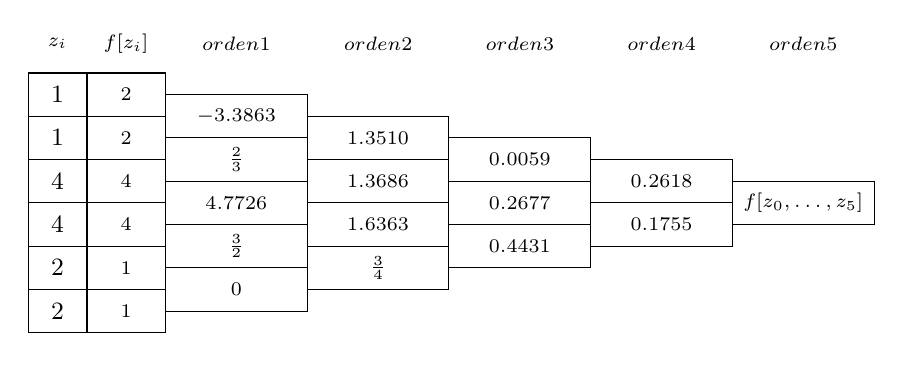
\begin{tikzpicture}[x=1cm,y=1cm]\path[use as bounding box] (0,-4.10) rectangle (11,0);
\node[font=\scriptsize] at (0.38,-.2) {$z_i$};
\node[font=\scriptsize] at (1.25,-.2) {$f[z_i]$};
\node[font=\scriptsize] at (2.65,-.2) {$\text{orden }1$};
\node[font=\scriptsize] at (4.45,-.2) {$\text{orden }2$};
\node[font=\scriptsize] at (6.25,-.2) {$\text{orden }3$};
\node[font=\scriptsize] at (8.05,-.2) {$\text{orden }4$};
\node[font=\scriptsize] at (9.85,-.2) {$\text{orden }5$};
\node[draw,minimum width=.75cm,minimum height=.55cm,font=\small,inner sep=1pt] at (.38,-0.85) {$1$};
\node[draw,minimum width=.75cm,minimum height=.55cm,font=\small,inner sep=1pt] at (.38,-1.4) {$1$};
\node[draw,minimum width=.75cm,minimum height=.55cm,font=\small,inner sep=1pt] at (.38,-1.9500000000000002) {$4$};
\node[draw,minimum width=.75cm,minimum height=.55cm,font=\small,inner sep=1pt] at (.38,-2.5) {$4$};
\node[draw,minimum width=.75cm,minimum height=.55cm,font=\small,inner sep=1pt] at (.38,-3.0500000000000003) {$2$};
\node[draw,minimum width=.75cm,minimum height=.55cm,font=\small,inner sep=1pt] at (.38,-3.6) {$2$};
\node[draw,minimum width=1cm,minimum height=.55cm,font=\scriptsize,inner sep=1pt] at (1.25,-0.85) {$2$};
\node[draw,minimum width=1cm,minimum height=.55cm,font=\scriptsize,inner sep=1pt] at (1.25,-1.4) {$2$};
\node[draw,minimum width=1cm,minimum height=.55cm,font=\scriptsize,inner sep=1pt] at (1.25,-1.9500000000000002) {$4$};
\node[draw,minimum width=1cm,minimum height=.55cm,font=\scriptsize,inner sep=1pt] at (1.25,-2.5) {$4$};
\node[draw,minimum width=1cm,minimum height=.55cm,font=\scriptsize,inner sep=1pt] at (1.25,-3.0500000000000003) {$1$};
\node[draw,minimum width=1cm,minimum height=.55cm,font=\scriptsize,inner sep=1pt] at (1.25,-3.6) {$1$};
\node[draw,minimum width=1.8cm,minimum height=.55cm,font=\scriptsize,inner sep=1pt] at (2.65,-1.125) {$-3.3863$};
\node[draw,minimum width=1.8cm,minimum height=.55cm,font=\scriptsize,inner sep=1pt] at (2.65,-1.6749999999999998) {$\frac23$};
\node[draw,minimum width=1.8cm,minimum height=.55cm,font=\scriptsize,inner sep=1pt] at (2.65,-2.225) {$4.7726$};
\node[draw,minimum width=1.8cm,minimum height=.55cm,font=\scriptsize,inner sep=1pt] at (2.65,-2.775) {$\frac32$};
\node[draw,minimum width=1.8cm,minimum height=.55cm,font=\scriptsize,inner sep=1pt] at (2.65,-3.325) {$0$};
\node[draw,minimum width=1.8cm,minimum height=.55cm,font=\scriptsize,inner sep=1pt] at (4.45,-1.4) {$1.3510$};
\node[draw,minimum width=1.8cm,minimum height=.55cm,font=\scriptsize,inner sep=1pt] at (4.45,-1.95) {$1.3686$};
\node[draw,minimum width=1.8cm,minimum height=.55cm,font=\scriptsize,inner sep=1pt] at (4.45,-2.5) {$1.6363$};
\node[draw,minimum width=1.8cm,minimum height=.55cm,font=\scriptsize,inner sep=1pt] at (4.45,-3.05) {$\frac34$};
\node[draw,minimum width=1.8cm,minimum height=.55cm,font=\scriptsize,inner sep=1pt] at (6.25,-1.675) {$0.0059$};
\node[draw,minimum width=1.8cm,minimum height=.55cm,font=\scriptsize,inner sep=1pt] at (6.25,-2.225) {$0.2677$};
\node[draw,minimum width=1.8cm,minimum height=.55cm,font=\scriptsize,inner sep=1pt] at (6.25,-2.7750000000000004) {$0.4431$};
\node[draw,minimum width=1.8cm,minimum height=.55cm,font=\scriptsize,inner sep=1pt] at (8.05,-1.9500000000000002) {$0.2618$};
\node[draw,minimum width=1.8cm,minimum height=.55cm,font=\scriptsize,inner sep=1pt] at (8.05,-2.5) {$0.1755$};
\node[draw,minimum width=1.8cm,minimum height=.55cm,font=\scriptsize,inner sep=1pt] at (9.85,-2.225) {$f[z_0,\ldots,z_5]$};
\end{tikzpicture}\end{center}\end{minipage}\par\scriptsize Los nodos repetidos son $1,1,4,4,2,2$.
\end{frame}
\begin{frame}[t]{Hermite: ejemplo}
\par\noindent\begin{minipage}[t][13mm][t]{\textwidth}\small\strut $f(x)=(x/2)^{x-2}$, $f\prime(x)=f(x)\big((x-2)/x+\ln(x/2)\big)$.\end{minipage}\par\nointerlineskip
\begin{minipage}[t]{\textwidth}\begin{center}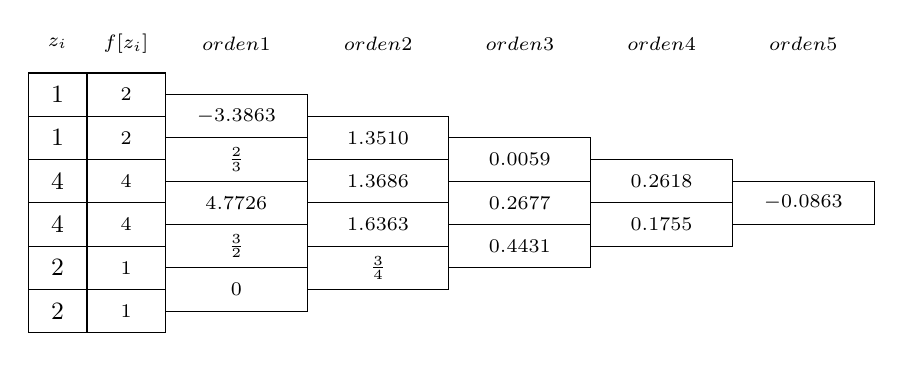
\begin{tikzpicture}[x=1cm,y=1cm]\path[use as bounding box] (0,-4.10) rectangle (11,0);
\node[font=\scriptsize] at (0.38,-.2) {$z_i$};
\node[font=\scriptsize] at (1.25,-.2) {$f[z_i]$};
\node[font=\scriptsize] at (2.65,-.2) {$\text{orden }1$};
\node[font=\scriptsize] at (4.45,-.2) {$\text{orden }2$};
\node[font=\scriptsize] at (6.25,-.2) {$\text{orden }3$};
\node[font=\scriptsize] at (8.05,-.2) {$\text{orden }4$};
\node[font=\scriptsize] at (9.85,-.2) {$\text{orden }5$};
\node[draw,minimum width=.75cm,minimum height=.55cm,font=\small,inner sep=1pt] at (.38,-0.85) {$1$};
\node[draw,minimum width=.75cm,minimum height=.55cm,font=\small,inner sep=1pt] at (.38,-1.4) {$1$};
\node[draw,minimum width=.75cm,minimum height=.55cm,font=\small,inner sep=1pt] at (.38,-1.9500000000000002) {$4$};
\node[draw,minimum width=.75cm,minimum height=.55cm,font=\small,inner sep=1pt] at (.38,-2.5) {$4$};
\node[draw,minimum width=.75cm,minimum height=.55cm,font=\small,inner sep=1pt] at (.38,-3.0500000000000003) {$2$};
\node[draw,minimum width=.75cm,minimum height=.55cm,font=\small,inner sep=1pt] at (.38,-3.6) {$2$};
\node[draw,minimum width=1cm,minimum height=.55cm,font=\scriptsize,inner sep=1pt] at (1.25,-0.85) {$2$};
\node[draw,minimum width=1cm,minimum height=.55cm,font=\scriptsize,inner sep=1pt] at (1.25,-1.4) {$2$};
\node[draw,minimum width=1cm,minimum height=.55cm,font=\scriptsize,inner sep=1pt] at (1.25,-1.9500000000000002) {$4$};
\node[draw,minimum width=1cm,minimum height=.55cm,font=\scriptsize,inner sep=1pt] at (1.25,-2.5) {$4$};
\node[draw,minimum width=1cm,minimum height=.55cm,font=\scriptsize,inner sep=1pt] at (1.25,-3.0500000000000003) {$1$};
\node[draw,minimum width=1cm,minimum height=.55cm,font=\scriptsize,inner sep=1pt] at (1.25,-3.6) {$1$};
\node[draw,minimum width=1.8cm,minimum height=.55cm,font=\scriptsize,inner sep=1pt] at (2.65,-1.125) {$-3.3863$};
\node[draw,minimum width=1.8cm,minimum height=.55cm,font=\scriptsize,inner sep=1pt] at (2.65,-1.6749999999999998) {$\frac23$};
\node[draw,minimum width=1.8cm,minimum height=.55cm,font=\scriptsize,inner sep=1pt] at (2.65,-2.225) {$4.7726$};
\node[draw,minimum width=1.8cm,minimum height=.55cm,font=\scriptsize,inner sep=1pt] at (2.65,-2.775) {$\frac32$};
\node[draw,minimum width=1.8cm,minimum height=.55cm,font=\scriptsize,inner sep=1pt] at (2.65,-3.325) {$0$};
\node[draw,minimum width=1.8cm,minimum height=.55cm,font=\scriptsize,inner sep=1pt] at (4.45,-1.4) {$1.3510$};
\node[draw,minimum width=1.8cm,minimum height=.55cm,font=\scriptsize,inner sep=1pt] at (4.45,-1.95) {$1.3686$};
\node[draw,minimum width=1.8cm,minimum height=.55cm,font=\scriptsize,inner sep=1pt] at (4.45,-2.5) {$1.6363$};
\node[draw,minimum width=1.8cm,minimum height=.55cm,font=\scriptsize,inner sep=1pt] at (4.45,-3.05) {$\frac34$};
\node[draw,minimum width=1.8cm,minimum height=.55cm,font=\scriptsize,inner sep=1pt] at (6.25,-1.675) {$0.0059$};
\node[draw,minimum width=1.8cm,minimum height=.55cm,font=\scriptsize,inner sep=1pt] at (6.25,-2.225) {$0.2677$};
\node[draw,minimum width=1.8cm,minimum height=.55cm,font=\scriptsize,inner sep=1pt] at (6.25,-2.7750000000000004) {$0.4431$};
\node[draw,minimum width=1.8cm,minimum height=.55cm,font=\scriptsize,inner sep=1pt] at (8.05,-1.9500000000000002) {$0.2618$};
\node[draw,minimum width=1.8cm,minimum height=.55cm,font=\scriptsize,inner sep=1pt] at (8.05,-2.5) {$0.1755$};
\node[draw,minimum width=1.8cm,minimum height=.55cm,font=\scriptsize,inner sep=1pt] at (9.85,-2.225) {$-0.0863$};
\end{tikzpicture}\end{center}\end{minipage}\par\scriptsize Los nodos repetidos son $1,1,4,4,2,2$.
\end{frame}
\begin{frame}[t]{Hermite: polinomio cúbico}
\par\noindent\begin{minipage}[t][13mm][t]{\textwidth}\small\strut $f(x)=(x/2)^{x-2}$, $f\prime(x)=f(x)\big((x-2)/x+\ln(x/2)\big)$.\end{minipage}\par\nointerlineskip
\begin{minipage}[t]{\textwidth}\begin{center}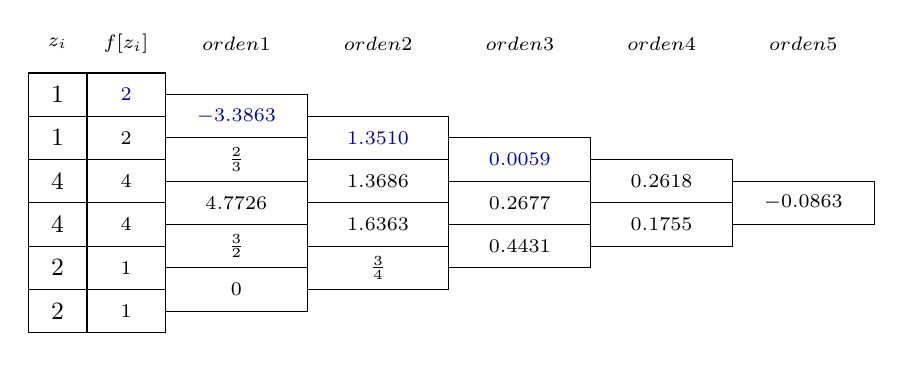
\begin{tikzpicture}[x=1cm,y=1cm]\path[use as bounding box] (0,-4.10) rectangle (11,0);
\node[font=\scriptsize] at (0.38,-.2) {$z_i$};
\node[font=\scriptsize] at (1.25,-.2) {$f[z_i]$};
\node[font=\scriptsize] at (2.65,-.2) {$\text{orden }1$};
\node[font=\scriptsize] at (4.45,-.2) {$\text{orden }2$};
\node[font=\scriptsize] at (6.25,-.2) {$\text{orden }3$};
\node[font=\scriptsize] at (8.05,-.2) {$\text{orden }4$};
\node[font=\scriptsize] at (9.85,-.2) {$\text{orden }5$};
\node[draw,minimum width=.75cm,minimum height=.55cm,font=\small,inner sep=1pt] at (.38,-0.85) {$1$};
\node[draw,minimum width=.75cm,minimum height=.55cm,font=\small,inner sep=1pt] at (.38,-1.4) {$1$};
\node[draw,minimum width=.75cm,minimum height=.55cm,font=\small,inner sep=1pt] at (.38,-1.9500000000000002) {$4$};
\node[draw,minimum width=.75cm,minimum height=.55cm,font=\small,inner sep=1pt] at (.38,-2.5) {$4$};
\node[draw,minimum width=.75cm,minimum height=.55cm,font=\small,inner sep=1pt] at (.38,-3.0500000000000003) {$2$};
\node[draw,minimum width=.75cm,minimum height=.55cm,font=\small,inner sep=1pt] at (.38,-3.6) {$2$};
\node[draw,minimum width=1cm,minimum height=.55cm,font=\scriptsize,inner sep=1pt,text=blue!70!black] at (1.25,-0.85) {$2$};
\node[draw,minimum width=1cm,minimum height=.55cm,font=\scriptsize,inner sep=1pt] at (1.25,-1.4) {$2$};
\node[draw,minimum width=1cm,minimum height=.55cm,font=\scriptsize,inner sep=1pt] at (1.25,-1.9500000000000002) {$4$};
\node[draw,minimum width=1cm,minimum height=.55cm,font=\scriptsize,inner sep=1pt] at (1.25,-2.5) {$4$};
\node[draw,minimum width=1cm,minimum height=.55cm,font=\scriptsize,inner sep=1pt] at (1.25,-3.0500000000000003) {$1$};
\node[draw,minimum width=1cm,minimum height=.55cm,font=\scriptsize,inner sep=1pt] at (1.25,-3.6) {$1$};
\node[draw,minimum width=1.8cm,minimum height=.55cm,font=\scriptsize,inner sep=1pt,text=blue!70!black] at (2.65,-1.125) {$-3.3863$};
\node[draw,minimum width=1.8cm,minimum height=.55cm,font=\scriptsize,inner sep=1pt] at (2.65,-1.6749999999999998) {$\frac23$};
\node[draw,minimum width=1.8cm,minimum height=.55cm,font=\scriptsize,inner sep=1pt] at (2.65,-2.225) {$4.7726$};
\node[draw,minimum width=1.8cm,minimum height=.55cm,font=\scriptsize,inner sep=1pt] at (2.65,-2.775) {$\frac32$};
\node[draw,minimum width=1.8cm,minimum height=.55cm,font=\scriptsize,inner sep=1pt] at (2.65,-3.325) {$0$};
\node[draw,minimum width=1.8cm,minimum height=.55cm,font=\scriptsize,inner sep=1pt,text=blue!70!black] at (4.45,-1.4) {$1.3510$};
\node[draw,minimum width=1.8cm,minimum height=.55cm,font=\scriptsize,inner sep=1pt] at (4.45,-1.95) {$1.3686$};
\node[draw,minimum width=1.8cm,minimum height=.55cm,font=\scriptsize,inner sep=1pt] at (4.45,-2.5) {$1.6363$};
\node[draw,minimum width=1.8cm,minimum height=.55cm,font=\scriptsize,inner sep=1pt] at (4.45,-3.05) {$\frac34$};
\node[draw,minimum width=1.8cm,minimum height=.55cm,font=\scriptsize,inner sep=1pt,text=blue!70!black] at (6.25,-1.675) {$0.0059$};
\node[draw,minimum width=1.8cm,minimum height=.55cm,font=\scriptsize,inner sep=1pt] at (6.25,-2.225) {$0.2677$};
\node[draw,minimum width=1.8cm,minimum height=.55cm,font=\scriptsize,inner sep=1pt] at (6.25,-2.7750000000000004) {$0.4431$};
\node[draw,minimum width=1.8cm,minimum height=.55cm,font=\scriptsize,inner sep=1pt] at (8.05,-1.9500000000000002) {$0.2618$};
\node[draw,minimum width=1.8cm,minimum height=.55cm,font=\scriptsize,inner sep=1pt] at (8.05,-2.5) {$0.1755$};
\node[draw,minimum width=1.8cm,minimum height=.55cm,font=\scriptsize,inner sep=1pt] at (9.85,-2.225) {$-0.0863$};
\end{tikzpicture}\end{center}\end{minipage}\par\scriptsize\[\begin{aligned}
H_3(x)\approx{}&2-3.386294(x-1)+1.350987(x-1)^2\\
&+0.005885(x-1)^2(x-4).
\end{aligned}\]\[f(3)=1.5,\quad H_3(3)\approx0.607821,\quad |f(3)-H_3(3)|\approx0.892179.\]
\end{frame}
\begin{frame}[t]{Hermite: polinomio de grado cinco}
\par\noindent\begin{minipage}[t][13mm][t]{\textwidth}\small\strut $f(x)=(x/2)^{x-2}$, $f\prime(x)=f(x)\big((x-2)/x+\ln(x/2)\big)$.\end{minipage}\par\nointerlineskip
\begin{minipage}[t]{\textwidth}\begin{center}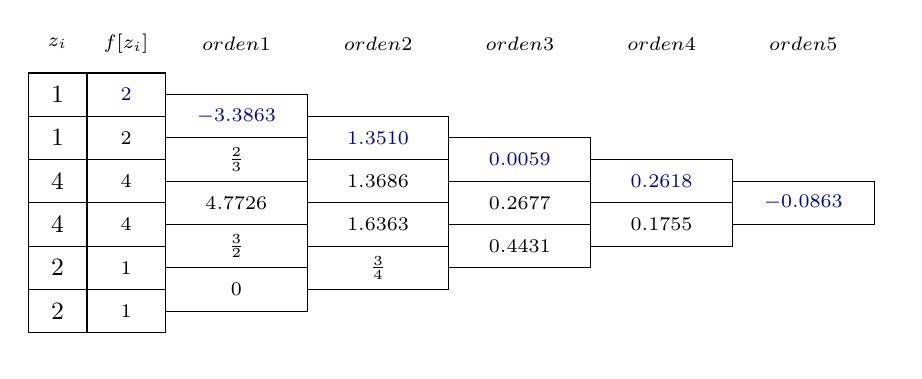
\begin{tikzpicture}[x=1cm,y=1cm]\path[use as bounding box] (0,-4.10) rectangle (11,0);
\node[font=\scriptsize] at (0.38,-.2) {$z_i$};
\node[font=\scriptsize] at (1.25,-.2) {$f[z_i]$};
\node[font=\scriptsize] at (2.65,-.2) {$\text{orden }1$};
\node[font=\scriptsize] at (4.45,-.2) {$\text{orden }2$};
\node[font=\scriptsize] at (6.25,-.2) {$\text{orden }3$};
\node[font=\scriptsize] at (8.05,-.2) {$\text{orden }4$};
\node[font=\scriptsize] at (9.85,-.2) {$\text{orden }5$};
\node[draw,minimum width=.75cm,minimum height=.55cm,font=\small,inner sep=1pt] at (.38,-0.85) {$1$};
\node[draw,minimum width=.75cm,minimum height=.55cm,font=\small,inner sep=1pt] at (.38,-1.4) {$1$};
\node[draw,minimum width=.75cm,minimum height=.55cm,font=\small,inner sep=1pt] at (.38,-1.9500000000000002) {$4$};
\node[draw,minimum width=.75cm,minimum height=.55cm,font=\small,inner sep=1pt] at (.38,-2.5) {$4$};
\node[draw,minimum width=.75cm,minimum height=.55cm,font=\small,inner sep=1pt] at (.38,-3.0500000000000003) {$2$};
\node[draw,minimum width=.75cm,minimum height=.55cm,font=\small,inner sep=1pt] at (.38,-3.6) {$2$};
\node[draw,minimum width=1cm,minimum height=.55cm,font=\scriptsize,inner sep=1pt,text=blue!70!black] at (1.25,-0.85) {$2$};
\node[draw,minimum width=1cm,minimum height=.55cm,font=\scriptsize,inner sep=1pt] at (1.25,-1.4) {$2$};
\node[draw,minimum width=1cm,minimum height=.55cm,font=\scriptsize,inner sep=1pt] at (1.25,-1.9500000000000002) {$4$};
\node[draw,minimum width=1cm,minimum height=.55cm,font=\scriptsize,inner sep=1pt] at (1.25,-2.5) {$4$};
\node[draw,minimum width=1cm,minimum height=.55cm,font=\scriptsize,inner sep=1pt] at (1.25,-3.0500000000000003) {$1$};
\node[draw,minimum width=1cm,minimum height=.55cm,font=\scriptsize,inner sep=1pt] at (1.25,-3.6) {$1$};
\node[draw,minimum width=1.8cm,minimum height=.55cm,font=\scriptsize,inner sep=1pt,text=blue!70!black] at (2.65,-1.125) {$-3.3863$};
\node[draw,minimum width=1.8cm,minimum height=.55cm,font=\scriptsize,inner sep=1pt] at (2.65,-1.6749999999999998) {$\frac23$};
\node[draw,minimum width=1.8cm,minimum height=.55cm,font=\scriptsize,inner sep=1pt] at (2.65,-2.225) {$4.7726$};
\node[draw,minimum width=1.8cm,minimum height=.55cm,font=\scriptsize,inner sep=1pt] at (2.65,-2.775) {$\frac32$};
\node[draw,minimum width=1.8cm,minimum height=.55cm,font=\scriptsize,inner sep=1pt] at (2.65,-3.325) {$0$};
\node[draw,minimum width=1.8cm,minimum height=.55cm,font=\scriptsize,inner sep=1pt,text=blue!70!black] at (4.45,-1.4) {$1.3510$};
\node[draw,minimum width=1.8cm,minimum height=.55cm,font=\scriptsize,inner sep=1pt] at (4.45,-1.95) {$1.3686$};
\node[draw,minimum width=1.8cm,minimum height=.55cm,font=\scriptsize,inner sep=1pt] at (4.45,-2.5) {$1.6363$};
\node[draw,minimum width=1.8cm,minimum height=.55cm,font=\scriptsize,inner sep=1pt] at (4.45,-3.05) {$\frac34$};
\node[draw,minimum width=1.8cm,minimum height=.55cm,font=\scriptsize,inner sep=1pt,text=blue!70!black] at (6.25,-1.675) {$0.0059$};
\node[draw,minimum width=1.8cm,minimum height=.55cm,font=\scriptsize,inner sep=1pt] at (6.25,-2.225) {$0.2677$};
\node[draw,minimum width=1.8cm,minimum height=.55cm,font=\scriptsize,inner sep=1pt] at (6.25,-2.7750000000000004) {$0.4431$};
\node[draw,minimum width=1.8cm,minimum height=.55cm,font=\scriptsize,inner sep=1pt,text=blue!70!black] at (8.05,-1.9500000000000002) {$0.2618$};
\node[draw,minimum width=1.8cm,minimum height=.55cm,font=\scriptsize,inner sep=1pt] at (8.05,-2.5) {$0.1755$};
\node[draw,minimum width=1.8cm,minimum height=.55cm,font=\scriptsize,inner sep=1pt,text=blue!70!black] at (9.85,-2.225) {$-0.0863$};
\end{tikzpicture}\end{center}\end{minipage}\par\scriptsize\begin{align*}
H_5(x)\approx{}&H_3(x)+0.261769(x-1)^2(x-4)^2\\
&-0.086276(x-1)^2(x-4)^2(x-2).
\end{align*}
\[H_5(3)\approx1.309795,\qquad |f(3)-H_5(3)|\approx0.190205.\]
\end{frame}
\begin{frame}[t]{Hermite: comparación gráfica}
\figura{hermite.png}{.90}{.78}
\end{frame}
\begin{frame}[t]{Polinomio intermedio de grado cuatro}
\par\noindent\begin{minipage}[t][13mm][t]{\textwidth}\small\strut $f(x)=(x/2)^{x-2}$, $f\prime(x)=f(x)\big((x-2)/x+\ln(x/2)\big)$.\end{minipage}\par\nointerlineskip
\begin{minipage}[t]{\textwidth}\begin{center}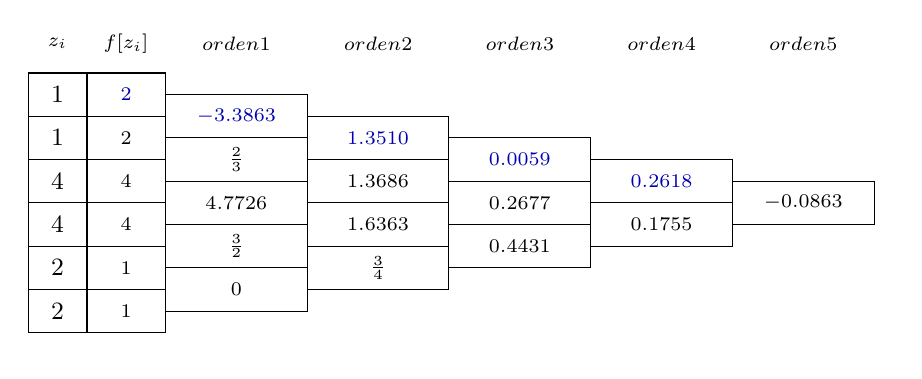
\begin{tikzpicture}[x=1cm,y=1cm]\path[use as bounding box] (0,-4.10) rectangle (11,0);
\node[font=\scriptsize] at (0.38,-.2) {$z_i$};
\node[font=\scriptsize] at (1.25,-.2) {$f[z_i]$};
\node[font=\scriptsize] at (2.65,-.2) {$\text{orden }1$};
\node[font=\scriptsize] at (4.45,-.2) {$\text{orden }2$};
\node[font=\scriptsize] at (6.25,-.2) {$\text{orden }3$};
\node[font=\scriptsize] at (8.05,-.2) {$\text{orden }4$};
\node[font=\scriptsize] at (9.85,-.2) {$\text{orden }5$};
\node[draw,minimum width=.75cm,minimum height=.55cm,font=\small,inner sep=1pt] at (.38,-0.85) {$1$};
\node[draw,minimum width=.75cm,minimum height=.55cm,font=\small,inner sep=1pt] at (.38,-1.4) {$1$};
\node[draw,minimum width=.75cm,minimum height=.55cm,font=\small,inner sep=1pt] at (.38,-1.9500000000000002) {$4$};
\node[draw,minimum width=.75cm,minimum height=.55cm,font=\small,inner sep=1pt] at (.38,-2.5) {$4$};
\node[draw,minimum width=.75cm,minimum height=.55cm,font=\small,inner sep=1pt] at (.38,-3.0500000000000003) {$2$};
\node[draw,minimum width=.75cm,minimum height=.55cm,font=\small,inner sep=1pt] at (.38,-3.6) {$2$};
\node[draw,minimum width=1cm,minimum height=.55cm,font=\scriptsize,inner sep=1pt,text=blue!70!black] at (1.25,-0.85) {$2$};
\node[draw,minimum width=1cm,minimum height=.55cm,font=\scriptsize,inner sep=1pt] at (1.25,-1.4) {$2$};
\node[draw,minimum width=1cm,minimum height=.55cm,font=\scriptsize,inner sep=1pt] at (1.25,-1.9500000000000002) {$4$};
\node[draw,minimum width=1cm,minimum height=.55cm,font=\scriptsize,inner sep=1pt] at (1.25,-2.5) {$4$};
\node[draw,minimum width=1cm,minimum height=.55cm,font=\scriptsize,inner sep=1pt] at (1.25,-3.0500000000000003) {$1$};
\node[draw,minimum width=1cm,minimum height=.55cm,font=\scriptsize,inner sep=1pt] at (1.25,-3.6) {$1$};
\node[draw,minimum width=1.8cm,minimum height=.55cm,font=\scriptsize,inner sep=1pt,text=blue!70!black] at (2.65,-1.125) {$-3.3863$};
\node[draw,minimum width=1.8cm,minimum height=.55cm,font=\scriptsize,inner sep=1pt] at (2.65,-1.6749999999999998) {$\frac23$};
\node[draw,minimum width=1.8cm,minimum height=.55cm,font=\scriptsize,inner sep=1pt] at (2.65,-2.225) {$4.7726$};
\node[draw,minimum width=1.8cm,minimum height=.55cm,font=\scriptsize,inner sep=1pt] at (2.65,-2.775) {$\frac32$};
\node[draw,minimum width=1.8cm,minimum height=.55cm,font=\scriptsize,inner sep=1pt] at (2.65,-3.325) {$0$};
\node[draw,minimum width=1.8cm,minimum height=.55cm,font=\scriptsize,inner sep=1pt,text=blue!70!black] at (4.45,-1.4) {$1.3510$};
\node[draw,minimum width=1.8cm,minimum height=.55cm,font=\scriptsize,inner sep=1pt] at (4.45,-1.95) {$1.3686$};
\node[draw,minimum width=1.8cm,minimum height=.55cm,font=\scriptsize,inner sep=1pt] at (4.45,-2.5) {$1.6363$};
\node[draw,minimum width=1.8cm,minimum height=.55cm,font=\scriptsize,inner sep=1pt] at (4.45,-3.05) {$\frac34$};
\node[draw,minimum width=1.8cm,minimum height=.55cm,font=\scriptsize,inner sep=1pt,text=blue!70!black] at (6.25,-1.675) {$0.0059$};
\node[draw,minimum width=1.8cm,minimum height=.55cm,font=\scriptsize,inner sep=1pt] at (6.25,-2.225) {$0.2677$};
\node[draw,minimum width=1.8cm,minimum height=.55cm,font=\scriptsize,inner sep=1pt] at (6.25,-2.7750000000000004) {$0.4431$};
\node[draw,minimum width=1.8cm,minimum height=.55cm,font=\scriptsize,inner sep=1pt,text=blue!70!black] at (8.05,-1.9500000000000002) {$0.2618$};
\node[draw,minimum width=1.8cm,minimum height=.55cm,font=\scriptsize,inner sep=1pt] at (8.05,-2.5) {$0.1755$};
\node[draw,minimum width=1.8cm,minimum height=.55cm,font=\scriptsize,inner sep=1pt] at (9.85,-2.225) {$-0.0863$};
\end{tikzpicture}\end{center}\end{minipage}\par\scriptsize
\[H_4(x)\approx H_3(x)+0.261769(x-1)^2(x-4)^2.\]
\[H_4(3)\approx1.654898,\quad f(3)=1.5,\quad |f(3)-H_4(3)|\approx0.154898.\]
Este polinomio de grado par interpola valores y parte de las derivadas; no satisface todas las condiciones del interpolante completo $H_5$.
\end{frame}
\begin{frame}[t]{Interpolación por splines}
La interpolación por partes usa polinomios en intervalos consecutivos.
\bigskip
En lugar de un único polinomio para todos los datos, se utilizan segmentos de grado bajo y se enlazan con condiciones de continuidad.
\bigskip
Así se reducen las oscilaciones que pueden aparecer al usar un interpolante global de grado alto.
\end{frame}
\begin{frame}[t]{Curvas spline}
En programas de diseño, las curvas spline se modelan mediante puntos de control.
\bigskip
Un spline polinómico está formado por polinomios enlazados en intervalos consecutivos.
\bigskip
En la interpolación, los puntos dados delimitan los intervalos y pertenecen a la curva.
\end{frame}
\begin{frame}[t]{Polinomios por intervalos}
Una función spline reúne varios polinomios, cada uno definido en un intervalo, que se unen con ciertas condiciones de continuidad.
\bigskip
Con muchos puntos, un interpolante global de grado alto puede presentar grandes oscilaciones.
\bigskip
Una alternativa es interpolar por intervalos con polinomios de grado bajo.
\end{frame}
\begin{frame}[t]{Splines lineales, cuadráticos y cúbicos}
\small Se utilizan polinomios lineales, cuadráticos o cúbicos. Trabajar por tramos de grado bajo simplifica el cálculo.
\begin{columns}\column{.32\textwidth}\figura{lineal.png}{1}{.50}\column{.32\textwidth}\figura{cuadratico.png}{1}{.50}\column{.32\textwidth}\figura{cubico.png}{1}{.50}\end{columns}
\end{frame}
\begin{frame}[t]{Splines lineales}
El spline lineal aproxima la curva entre cada par de nodos mediante una recta.\figura{ave-lineal.png}{.78}{.65}
\end{frame}
\begin{frame}[t]{Splines cuadráticos}
El spline cuadrático puede imponer continuidad de la primera derivada en los puntos de unión.
\bigskip
El polinomio de un intervalo termina con la misma pendiente con la que comienza el siguiente.
\bigskip
Se elimina así la sensación de recta quebrada.
\end{frame}
\begin{frame}[t]{Splines cúbicos}
\small El spline cúbico añade continuidad de la segunda derivada en los puntos de unión. La curva resulta más suave.\figura{ave-spline.png}{.78}{.66}
\end{frame}
\begin{frame}[t]{Spline cúbico interpolante}
\small Dados $x_0<x_1<\cdots<x_n$, un spline cúbico $S$ cumple:
\begin{columns}[T]\column{.66\textwidth}
\[S(x)=S_i(x),\quad x\in[x_i,x_{i+1}],\quad i=0,\ldots,n-1.\]
Cada $S_i$ es un polinomio de grado $\le3$ y
\[S(x_i)=f(x_i),\quad i=0,\ldots,n.\]
En los enlaces, para $i=0,\ldots,n-2$:
\begin{align*}S_i(x_{i+1})&=S_{i+1}(x_{i+1}),\\
S_i'(x_{i+1})&=S_{i+1}'(x_{i+1}),\\
S_i''(x_{i+1})&=S_{i+1}''(x_{i+1}).\end{align*}
\column{.32\textwidth}\figura{nodos.png}{1}{.20}\figura{tramos.png}{1}{.20}\figura{enlaces.png}{1}{.20}\end{columns}
\end{frame}
\begin{frame}[t]{Polinomios de los tramos}
\small
\[S_i(x)=a_i+b_i(x-x_i)+c_i(x-x_i)^2+d_i(x-x_i)^3.\]
Para los primeros y el último tramo:
\begin{align*}
S_0(x)&=a_0+b_0(x-x_0)+c_0(x-x_0)^2+d_0(x-x_0)^3,\\
S_1(x)&=a_1+b_1(x-x_1)+c_1(x-x_1)^2+d_1(x-x_1)^3,\\
&\ \vdots\\
S_{n-1}(x)&=a_{n-1}+b_{n-1}(x-x_{n-1})\\
&\quad+c_{n-1}(x-x_{n-1})^2+d_{n-1}(x-x_{n-1})^3.
\end{align*}
\end{frame}
\begin{frame}[t]{Condiciones en los extremos}
Dos tipos de condiciones para los splines cúbicos:
\begin{itemize}
\item \textbf{Spline natural}: segunda derivada nula en los extremos.
\[S''(x_0)=0,\qquad S''(x_n)=0.\]
\item \textbf{Spline sujeto} (extremo cortado): pendientes prescritas.
\[S'(x_0)=f'(x_0),\qquad S'(x_n)=f'(x_n).\]
\end{itemize}
\end{frame}
\begin{frame}[t]{Spline cúbico natural}
Consideraremos el spline natural por su simplicidad.
\bigskip
Para calcular los coeficientes de sus polinomios hay que resolver un sistema de ecuaciones.
\bigskip
Las condiciones naturales son $c_0=c_n=0$, porque $S''(x_i)=2c_i$.
\end{frame}
\begin{frame}[t]{Spline natural: fórmulas}
\begin{columns}[T]\column{.49\textwidth}\scriptsize\begin{align*}
h_i&=x_{i+1}-x_i,\qquad a_i=f(x_i),\\
d_i&=\frac{c_{i+1}-c_i}{3h_i},\\
b_i&=\frac{a_{i+1}-a_i}{h_i}-\frac{h_i}{3}(2c_i+c_{i+1}).
\end{align*}\[c_0=c_n=0.\]\column{.49\textwidth}\begin{minipage}[t]{\textwidth}\begingroup\scriptsize\setlength{\tabcolsep}{2pt}\begin{center}\begin{tabular}{|C{.12\textwidth}|C{.12\textwidth}|C{.12\textwidth}|C{.12\textwidth}|C{.12\textwidth}|C{.12\textwidth}|}\hline
\rule[-2mm]{0pt}{6mm}$x_i$&$h_i$&$a_i$&$b_i$&$c_i$&$d_i$\\\hline
\rule[-2.5mm]{0pt}{6mm}$x_0$&$h_0$&$a_0$&$b_0$&$0$&$d_0$\\\hline
\rule[-2.5mm]{0pt}{6mm}$x_1$&$h_1$&$a_1$&$b_1$&$c_1$&$d_1$\\\hline
\rule[-2.5mm]{0pt}{6mm}$\vdots$&$\vdots$&$\vdots$&$\vdots$&$\vdots$&$\vdots$\\\hline
\rule[-2.5mm]{0pt}{6mm}$x_{n-1}$&$h_{n-1}$&$a_{n-1}$&$b_{n-1}$&$c_{n-1}$&$d_{n-1}$\\\hline
\rule[-2.5mm]{0pt}{6mm}$x_n$& &$a_n$& &$0$& \\\hline
\end{tabular}\end{center}\endgroup\end{minipage}\par
\end{columns}\scriptsize
\[\underbrace{\begin{pmatrix}
m_{11}&m_{12}&0&\cdots\\
m_{21}&m_{22}&m_{23}&\cdots\\
\vdots&\ddots&\ddots&\ddots\\
\cdots&0&m_{n-1,n-2}&m_{n-1,n-1}
\end{pmatrix}}_{M}
\begin{pmatrix}c_1\\c_2\\\vdots\\c_{n-1}\end{pmatrix}
=\begin{pmatrix}v_1\\v_2\\\vdots\\v_{n-1}\end{pmatrix},\qquad \boldsymbol c=M^{-1}\boldsymbol v.\]
\scriptsize
\[m_{ii}=2(h_{i-1}+h_i),\quad m_{i,i-1}=h_{i-1},\quad m_{i,i+1}=h_i.\]
\[v_i=3\frac{a_{i+1}-a_i}{h_i}-3\frac{a_i-a_{i-1}}{h_{i-1}}.\]
\end{frame}
\begin{frame}[t]{Spline natural: ejemplo}
\par\noindent\begin{minipage}[t][13mm][t]{\textwidth}\small\strut $f(x)=(x/2)^{x-2}$; nodos $1,2,4$.\end{minipage}\par\nointerlineskip
\begin{columns}[T]\column{.44\textwidth}\scriptsize\begin{align*}
h_i&=x_{i+1}-x_i,\qquad a_i=f(x_i),\\
d_i&=\frac{c_{i+1}-c_i}{3h_i},\\
b_i&=\frac{a_{i+1}-a_i}{h_i}-\frac{h_i}{3}(2c_i+c_{i+1}).
\end{align*}\scriptsize\[c_0=c_2=0,\qquad c_1=m_{11}^{-1}v_1.\]\column{.54\textwidth}\begin{minipage}[t]{\textwidth}\begingroup\scriptsize\setlength{\tabcolsep}{2pt}\begin{center}\begin{tabular}{|C{.12\textwidth}|C{.12\textwidth}|C{.12\textwidth}|C{.12\textwidth}|C{.12\textwidth}|C{.12\textwidth}|}\hline
\rule[-2mm]{0pt}{6mm}$x_i$&$h_i$&$a_i$&$b_i$&$c_i$&$d_i$\\\hline
\rule[-2.5mm]{0pt}{7mm}$x_0$&$h_0$&$a_0$&$b_0$&$0$&$d_0$\\\hline
\rule[-2.5mm]{0pt}{7mm}$x_1$&$h_1$&$a_1$&$b_1$&$c_1$&$d_1$\\\hline
\rule[-2.5mm]{0pt}{7mm}$x_2$&&$a_2$&&$0$&\\\hline
\end{tabular}\end{center}\endgroup\end{minipage}\par
\end{columns}
\end{frame}
\begin{frame}[t]{Spline natural: ejemplo}
\par\noindent\begin{minipage}[t][13mm][t]{\textwidth}\small\strut $f(x)=(x/2)^{x-2}$; nodos $1,2,4$.\end{minipage}\par\nointerlineskip
\begin{columns}[T]\column{.44\textwidth}\scriptsize\begin{align*}
h_i&=x_{i+1}-x_i,\qquad a_i=f(x_i),\\
d_i&=\frac{c_{i+1}-c_i}{3h_i},\\
b_i&=\frac{a_{i+1}-a_i}{h_i}-\frac{h_i}{3}(2c_i+c_{i+1}).
\end{align*}\scriptsize\[c_0=c_2=0,\qquad c_1=m_{11}^{-1}v_1.\]\column{.54\textwidth}\begin{minipage}[t]{\textwidth}\begingroup\scriptsize\setlength{\tabcolsep}{2pt}\begin{center}\begin{tabular}{|C{.12\textwidth}|C{.12\textwidth}|C{.12\textwidth}|C{.12\textwidth}|C{.12\textwidth}|C{.12\textwidth}|}\hline
\rule[-2mm]{0pt}{6mm}$x_i$&$h_i$&$a_i$&$b_i$&$c_i$&$d_i$\\\hline
\rule[-2.5mm]{0pt}{7mm}$1$&$1$&$2$&$b_0$&$0$&$d_0$\\\hline
\rule[-2.5mm]{0pt}{7mm}$2$&$2$&$1$&$b_1$&$c_1$&$d_1$\\\hline
\rule[-2.5mm]{0pt}{7mm}$4$&&$4$&&$0$&\\\hline
\end{tabular}\end{center}\endgroup\end{minipage}\par
\scriptsize\[m_{11}=2(h_0+h_1),\]\[v_1=3\frac{a_2-a_1}{h_1}-3\frac{a_1-a_0}{h_0}.\]\end{columns}
\end{frame}
\begin{frame}[t]{Spline natural: ejemplo}
\par\noindent\begin{minipage}[t][13mm][t]{\textwidth}\small\strut $f(x)=(x/2)^{x-2}$; nodos $1,2,4$.\end{minipage}\par\nointerlineskip
\begin{columns}[T]\column{.44\textwidth}\scriptsize\begin{align*}
h_i&=x_{i+1}-x_i,\qquad a_i=f(x_i),\\
d_i&=\frac{c_{i+1}-c_i}{3h_i},\\
b_i&=\frac{a_{i+1}-a_i}{h_i}-\frac{h_i}{3}(2c_i+c_{i+1}).
\end{align*}\scriptsize\[m_{11}=2(1+2)=6.\]\[v_1=3\frac{4-1}{2}-3\frac{1-2}{1}=\frac{15}{2}.\]\column{.54\textwidth}\begin{minipage}[t]{\textwidth}\begingroup\scriptsize\setlength{\tabcolsep}{2pt}\begin{center}\begin{tabular}{|C{.12\textwidth}|C{.12\textwidth}|C{.12\textwidth}|C{.12\textwidth}|C{.12\textwidth}|C{.12\textwidth}|}\hline
\rule[-2mm]{0pt}{6mm}$x_i$&$h_i$&$a_i$&$b_i$&$c_i$&$d_i$\\\hline
\rule[-2.5mm]{0pt}{7mm}$1$&$1$&$2$&$b_0$&$0$&$d_0$\\\hline
\rule[-2.5mm]{0pt}{7mm}$2$&$2$&$1$&$b_1$&$c_1$&$d_1$\\\hline
\rule[-2.5mm]{0pt}{7mm}$4$&&$4$&&$0$&\\\hline
\end{tabular}\end{center}\endgroup\end{minipage}\par
\scriptsize\[c_0=c_2=0,\quad c_1=\frac16\cdot\frac{15}{2}.\]\end{columns}
\end{frame}
\begin{frame}[t]{Spline natural: ejemplo}
\par\noindent\begin{minipage}[t][13mm][t]{\textwidth}\small\strut $f(x)=(x/2)^{x-2}$; nodos $1,2,4$.\end{minipage}\par\nointerlineskip
\begin{columns}[T]\column{.44\textwidth}\scriptsize\begin{align*}
h_i&=x_{i+1}-x_i,\qquad a_i=f(x_i),\\
d_i&=\frac{c_{i+1}-c_i}{3h_i},\\
b_i&=\frac{a_{i+1}-a_i}{h_i}-\frac{h_i}{3}(2c_i+c_{i+1}).
\end{align*}\scriptsize\[c_0=c_2=0,\qquad c_1=\frac54.\]\column{.54\textwidth}\begin{minipage}[t]{\textwidth}\begingroup\scriptsize\setlength{\tabcolsep}{2pt}\begin{center}\begin{tabular}{|C{.12\textwidth}|C{.12\textwidth}|C{.12\textwidth}|C{.12\textwidth}|C{.12\textwidth}|C{.12\textwidth}|}\hline
\rule[-2mm]{0pt}{6mm}$x_i$&$h_i$&$a_i$&$b_i$&$c_i$&$d_i$\\\hline
\rule[-2.5mm]{0pt}{7mm}$1$&$1$&$2$&$b_0$&$0$&$d_0$\\\hline
\rule[-2.5mm]{0pt}{7mm}$2$&$2$&$1$&$b_1$&$\frac{5}{4}$&$d_1$\\\hline
\rule[-2.5mm]{0pt}{7mm}$4$&&$4$&&$0$&\\\hline
\end{tabular}\end{center}\endgroup\end{minipage}\par
\scriptsize\[c_1=6^{-1}\cdot\frac{15}{2}=\frac54.\]\end{columns}
\end{frame}
\begin{frame}[t]{Spline natural: ejemplo}
\par\noindent\begin{minipage}[t][13mm][t]{\textwidth}\small\strut $f(x)=(x/2)^{x-2}$; nodos $1,2,4$.\end{minipage}\par\nointerlineskip
\begin{columns}[T]\column{.44\textwidth}\scriptsize\begin{align*}
h_i&=x_{i+1}-x_i,\qquad a_i=f(x_i),\\
d_i&=\frac{c_{i+1}-c_i}{3h_i},\\
b_i&=\frac{a_{i+1}-a_i}{h_i}-\frac{h_i}{3}(2c_i+c_{i+1}).
\end{align*}\scriptsize\[S_i(x)=a_i+b_i(x-x_i)\]\[{}+c_i(x-x_i)^2+d_i(x-x_i)^3.\]\column{.54\textwidth}\begin{minipage}[t]{\textwidth}\begingroup\scriptsize\setlength{\tabcolsep}{2pt}\begin{center}\begin{tabular}{|C{.12\textwidth}|C{.12\textwidth}|C{.12\textwidth}|C{.12\textwidth}|C{.12\textwidth}|C{.12\textwidth}|}\hline
\rule[-2mm]{0pt}{6mm}$x_i$&$h_i$&$a_i$&$b_i$&$c_i$&$d_i$\\\hline
\rule[-2.5mm]{0pt}{7mm}$1$&$1$&$2$&$-\frac{17}{12}$&$0$&$\frac{5}{12}$\\\hline
\rule[-2.5mm]{0pt}{7mm}$2$&$2$&$1$&$-\frac{1}{6}$&$\frac{5}{4}$&$-\frac{5}{24}$\\\hline
\rule[-2.5mm]{0pt}{7mm}$4$&&$4$&&$0$&\\\hline
\end{tabular}\end{center}\endgroup\end{minipage}\par
\end{columns}
\end{frame}
\begin{frame}[t]{Spline natural: tres nodos}
\par\noindent\begin{minipage}[t][13mm][t]{\textwidth}\small\strut $f(x)=(x/2)^{x-2}$; nodos $1,2,4$.\end{minipage}\par\nointerlineskip
\begin{columns}[T]\column{.49\textwidth}\figura{spline3.png}{1}{.35}\column{.49\textwidth}\begin{minipage}[t]{\textwidth}\begingroup\scriptsize\setlength{\tabcolsep}{2pt}\begin{center}\begin{tabular}{|C{.12\textwidth}|C{.12\textwidth}|C{.12\textwidth}|C{.12\textwidth}|C{.12\textwidth}|C{.12\textwidth}|}\hline
\rule[-2mm]{0pt}{6mm}$x_i$&$h_i$&$a_i$&$b_i$&$c_i$&$d_i$\\\hline
\rule[-2.5mm]{0pt}{7mm}$1$&$1$&$2$&$-\frac{17}{12}$&$0$&$\frac{5}{12}$\\\hline
\rule[-2.5mm]{0pt}{7mm}$2$&$2$&$1$&$-\frac{1}{6}$&$\frac{5}{4}$&$-\frac{5}{24}$\\\hline
\rule[-2.5mm]{0pt}{7mm}$4$&&$4$&&$0$&\\\hline
\end{tabular}\end{center}\endgroup\end{minipage}\par
\end{columns}\small
\[S(x)=\begin{cases}
2-\frac{17}{12}(x-1)+\frac5{12}(x-1)^3,&x\in[1,2],\\[2mm]
1-\frac16(x-2)+\frac54(x-2)^2-\frac5{24}(x-2)^3,&x\in[2,4].
\end{cases}\]
\end{frame}
\begin{frame}[t]{Spline natural: ejemplo}
\par\noindent\begin{minipage}[t][13mm][t]{\textwidth}\small\strut $f(x)=(x/2)^{x-2}$; nodos $1,2,3,4,5$.\end{minipage}\par\nointerlineskip
\begin{columns}[T]\column{.44\textwidth}\scriptsize\begin{align*}
h_i&=x_{i+1}-x_i,\qquad a_i=f(x_i),\\
d_i&=\frac{c_{i+1}-c_i}{3h_i},\\
b_i&=\frac{a_{i+1}-a_i}{h_i}-\frac{h_i}{3}(2c_i+c_{i+1}).
\end{align*}\scriptsize\[\begin{pmatrix}c_1\\c_2\\c_3\end{pmatrix}=M^{-1}\begin{pmatrix}v_1\\v_2\\v_3\end{pmatrix},\quad c_0=c_4=0.\]\column{.54\textwidth}\begin{minipage}[t]{\textwidth}\begingroup\scriptsize\setlength{\tabcolsep}{2pt}\begin{center}\begin{tabular}{|C{.12\textwidth}|C{.12\textwidth}|C{.12\textwidth}|C{.12\textwidth}|C{.12\textwidth}|C{.12\textwidth}|}\hline
\rule[-2mm]{0pt}{6mm}$x_i$&$h_i$&$a_i$&$b_i$&$c_i$&$d_i$\\\hline
\rule[-2.5mm]{0pt}{7mm}$x_0$&$h_0$&$a_0$&$b_0$&$0$&$d_0$\\\hline
\rule[-2.5mm]{0pt}{7mm}$x_1$&$h_1$&$a_1$&$b_1$&$c_1$&$d_1$\\\hline
\rule[-2.5mm]{0pt}{7mm}$x_2$&$h_2$&$a_2$&$b_2$&$c_2$&$d_2$\\\hline
\rule[-2.5mm]{0pt}{7mm}$x_3$&$h_3$&$a_3$&$b_3$&$c_3$&$d_3$\\\hline
\rule[-2.5mm]{0pt}{7mm}$x_4$&&$a_4$&&$0$&\\\hline
\end{tabular}\end{center}\endgroup\end{minipage}\par
\end{columns}
\end{frame}
\begin{frame}[t]{Spline natural: ejemplo}
\par\noindent\begin{minipage}[t][13mm][t]{\textwidth}\small\strut $f(x)=(x/2)^{x-2}$; nodos $1,2,3,4,5$.\end{minipage}\par\nointerlineskip
\begin{columns}[T]\column{.44\textwidth}\scriptsize\begin{align*}
h_i&=x_{i+1}-x_i,\qquad a_i=f(x_i),\\
d_i&=\frac{c_{i+1}-c_i}{3h_i},\\
b_i&=\frac{a_{i+1}-a_i}{h_i}-\frac{h_i}{3}(2c_i+c_{i+1}).
\end{align*}\scriptsize\[\begin{pmatrix}c_1\\c_2\\c_3\end{pmatrix}=M^{-1}\begin{pmatrix}v_1\\v_2\\v_3\end{pmatrix},\quad c_0=c_4=0.\]\column{.54\textwidth}\begin{minipage}[t]{\textwidth}\begingroup\scriptsize\setlength{\tabcolsep}{2pt}\begin{center}\begin{tabular}{|C{.12\textwidth}|C{.12\textwidth}|C{.12\textwidth}|C{.12\textwidth}|C{.12\textwidth}|C{.12\textwidth}|}\hline
\rule[-2mm]{0pt}{6mm}$x_i$&$h_i$&$a_i$&$b_i$&$c_i$&$d_i$\\\hline
\rule[-2.5mm]{0pt}{7mm}$1$&$1$&$2$&$b_0$&$0$&$d_0$\\\hline
\rule[-2.5mm]{0pt}{7mm}$2$&$1$&$1$&$b_1$&$c_1$&$d_1$\\\hline
\rule[-2.5mm]{0pt}{7mm}$3$&$1$&$\frac{3}{2}$&$b_2$&$c_2$&$d_2$\\\hline
\rule[-2.5mm]{0pt}{7mm}$4$&$1$&$4$&$b_3$&$c_3$&$d_3$\\\hline
\rule[-2.5mm]{0pt}{7mm}$5$&&$\frac{125}{8}$&&$0$&\\\hline
\end{tabular}\end{center}\endgroup\end{minipage}\par
\end{columns}
\end{frame}
\begin{frame}[t]{Spline natural: ejemplo}
\par\noindent\begin{minipage}[t][13mm][t]{\textwidth}\small\strut $f(x)=(x/2)^{x-2}$; nodos $1,2,3,4,5$.\end{minipage}\par\nointerlineskip
\begin{columns}[T]\column{.44\textwidth}\scriptsize\begin{align*}
h_i&=x_{i+1}-x_i,\qquad a_i=f(x_i),\\
d_i&=\frac{c_{i+1}-c_i}{3h_i},\\
b_i&=\frac{a_{i+1}-a_i}{h_i}-\frac{h_i}{3}(2c_i+c_{i+1}).
\end{align*}\scriptsize\[\begin{pmatrix}c_1\\c_2\\c_3\end{pmatrix}=\begin{pmatrix}4&1&0\\1&4&1\\0&1&4\end{pmatrix}^{-1}\begin{pmatrix}9/2\\6\\219/8\end{pmatrix}.\]\column{.54\textwidth}\begin{minipage}[t]{\textwidth}\begingroup\scriptsize\setlength{\tabcolsep}{2pt}\begin{center}\begin{tabular}{|C{.12\textwidth}|C{.12\textwidth}|C{.12\textwidth}|C{.12\textwidth}|C{.12\textwidth}|C{.12\textwidth}|}\hline
\rule[-2mm]{0pt}{6mm}$x_i$&$h_i$&$a_i$&$b_i$&$c_i$&$d_i$\\\hline
\rule[-2.5mm]{0pt}{7mm}$1$&$1$&$2$&$b_0$&$0$&$d_0$\\\hline
\rule[-2.5mm]{0pt}{7mm}$2$&$1$&$1$&$b_1$&$c_1$&$d_1$\\\hline
\rule[-2.5mm]{0pt}{7mm}$3$&$1$&$\frac{3}{2}$&$b_2$&$c_2$&$d_2$\\\hline
\rule[-2.5mm]{0pt}{7mm}$4$&$1$&$4$&$b_3$&$c_3$&$d_3$\\\hline
\rule[-2.5mm]{0pt}{7mm}$5$&&$\frac{125}{8}$&&$0$&\\\hline
\end{tabular}\end{center}\endgroup\end{minipage}\par
\end{columns}
\end{frame}
\begin{frame}[t]{Spline natural: ejemplo}
\par\noindent\begin{minipage}[t][13mm][t]{\textwidth}\small\strut $f(x)=(x/2)^{x-2}$; nodos $1,2,3,4,5$.\end{minipage}\par\nointerlineskip
\begin{columns}[T]\column{.44\textwidth}\scriptsize\begin{align*}
h_i&=x_{i+1}-x_i,\qquad a_i=f(x_i),\\
d_i&=\frac{c_{i+1}-c_i}{3h_i},\\
b_i&=\frac{a_{i+1}-a_i}{h_i}-\frac{h_i}{3}(2c_i+c_{i+1}).
\end{align*}\scriptsize\[\begin{pmatrix}c_1\\c_2\\c_3\end{pmatrix}=\begin{pmatrix}4&1&0\\1&4&1\\0&1&4\end{pmatrix}^{-1}\begin{pmatrix}9/2\\6\\219/8\end{pmatrix}.\]\column{.54\textwidth}\begin{minipage}[t]{\textwidth}\begingroup\scriptsize\setlength{\tabcolsep}{2pt}\begin{center}\begin{tabular}{|C{.12\textwidth}|C{.12\textwidth}|C{.12\textwidth}|C{.12\textwidth}|C{.12\textwidth}|C{.12\textwidth}|}\hline
\rule[-2mm]{0pt}{6mm}$x_i$&$h_i$&$a_i$&$b_i$&$c_i$&$d_i$\\\hline
\rule[-2.5mm]{0pt}{7mm}$1$&$1$&$2$&$b_0$&$0$&$d_0$\\\hline
\rule[-2.5mm]{0pt}{7mm}$2$&$1$&$1$&$b_1$&$c_1$&$d_1$\\\hline
\rule[-2.5mm]{0pt}{7mm}$3$&$1$&$\frac{3}{2}$&$b_2$&$c_2$&$d_2$\\\hline
\rule[-2.5mm]{0pt}{7mm}$4$&$1$&$4$&$b_3$&$c_3$&$d_3$\\\hline
\rule[-2.5mm]{0pt}{7mm}$5$&&$\frac{125}{8}$&&$0$&\\\hline
\end{tabular}\end{center}\endgroup\end{minipage}\par
\scriptsize\[M^{-1}=\begin{pmatrix}15/56&-1/14&1/56\\-1/14&2/7&-1/14\\1/56&-1/14&15/56\end{pmatrix}.\]\end{columns}
\end{frame}
\begin{frame}[t]{Spline natural: ejemplo}
\par\noindent\begin{minipage}[t][13mm][t]{\textwidth}\small\strut $f(x)=(x/2)^{x-2}$; nodos $1,2,3,4,5$.\end{minipage}\par\nointerlineskip
\begin{columns}[T]\column{.44\textwidth}\scriptsize\begin{align*}
h_i&=x_{i+1}-x_i,\qquad a_i=f(x_i),\\
d_i&=\frac{c_{i+1}-c_i}{3h_i},\\
b_i&=\frac{a_{i+1}-a_i}{h_i}-\frac{h_i}{3}(2c_i+c_{i+1}).
\end{align*}\scriptsize\[\begin{pmatrix}c_1\\c_2\\c_3\end{pmatrix}=\begin{pmatrix}81/64\\-9/16\\447/64\end{pmatrix}.\]\column{.54\textwidth}\begin{minipage}[t]{\textwidth}\begingroup\scriptsize\setlength{\tabcolsep}{2pt}\begin{center}\begin{tabular}{|C{.12\textwidth}|C{.12\textwidth}|C{.12\textwidth}|C{.12\textwidth}|C{.12\textwidth}|C{.12\textwidth}|}\hline
\rule[-2mm]{0pt}{6mm}$x_i$&$h_i$&$a_i$&$b_i$&$c_i$&$d_i$\\\hline
\rule[-2.5mm]{0pt}{7mm}$1$&$1$&$2$&$b_0$&$0$&$d_0$\\\hline
\rule[-2.5mm]{0pt}{7mm}$2$&$1$&$1$&$b_1$&$\frac{81}{64}$&$d_1$\\\hline
\rule[-2.5mm]{0pt}{7mm}$3$&$1$&$\frac{3}{2}$&$b_2$&$-\frac{9}{16}$&$d_2$\\\hline
\rule[-2.5mm]{0pt}{7mm}$4$&$1$&$4$&$b_3$&$\frac{447}{64}$&$d_3$\\\hline
\rule[-2.5mm]{0pt}{7mm}$5$&&$\frac{125}{8}$&&$0$&\\\hline
\end{tabular}\end{center}\endgroup\end{minipage}\par
\end{columns}
\end{frame}
\begin{frame}[t]{Spline natural: coeficientes}
\par\noindent\begin{minipage}[t][13mm][t]{\textwidth}\small\strut $f(x)=(x/2)^{x-2}$; nodos $1,2,3,4,5$.\end{minipage}\par\nointerlineskip
\begin{minipage}[t]{\textwidth}\begingroup\scriptsize\setlength{\tabcolsep}{2pt}\begin{center}\begin{tabular}{|C{.12\textwidth}|C{.12\textwidth}|C{.12\textwidth}|C{.12\textwidth}|C{.12\textwidth}|C{.12\textwidth}|}\hline
\rule[-2mm]{0pt}{6mm}$x_i$&$h_i$&$a_i$&$b_i$&$c_i$&$d_i$\\\hline
\rule[-2.5mm]{0pt}{8mm}$1$&$1$&$2$&$-\frac{91}{64}$&$0$&$\frac{27}{64}$\\\hline
\rule[-2.5mm]{0pt}{8mm}$2$&$1$&$1$&$-\frac{5}{32}$&$\frac{81}{64}$&$-\frac{39}{64}$\\\hline
\rule[-2.5mm]{0pt}{8mm}$3$&$1$&$\frac{3}{2}$&$\frac{35}{64}$&$-\frac{9}{16}$&$\frac{161}{64}$\\\hline
\rule[-2.5mm]{0pt}{8mm}$4$&$1$&$4$&$\frac{223}{32}$&$\frac{447}{64}$&$-\frac{149}{64}$\\\hline
\rule[-2.5mm]{0pt}{8mm}$5$&&$\frac{125}{8}$&&$0$&\\\hline
\end{tabular}\end{center}\endgroup\end{minipage}\par
\[S_i(x)=a_i+b_i(x-x_i)+c_i(x-x_i)^2+d_i(x-x_i)^3.\]
\end{frame}
\begin{frame}[t]{Spline natural: expresión por tramos}
\small
\begin{align*}
x\in[1,2]:\quad S_0(x)&=2-\tfrac{91}{64}(x-1)+\tfrac{27}{64}(x-1)^3,\\[3mm]
x\in[2,3]:\quad S_1(x)&=1-\tfrac5{32}(x-2)+\tfrac{81}{64}(x-2)^2\\
&\quad-\tfrac{39}{64}(x-2)^3,\\[3mm]
x\in[3,4]:\quad S_2(x)&=\tfrac32+\tfrac{35}{64}(x-3)-\tfrac9{16}(x-3)^2\\
&\quad+\tfrac{161}{64}(x-3)^3,\\[3mm]
x\in[4,5]:\quad S_3(x)&=4+\tfrac{223}{32}(x-4)+\tfrac{447}{64}(x-4)^2\\
&\quad-\tfrac{149}{64}(x-4)^3.
\end{align*}
\end{frame}
\begin{frame}[t]{Spline natural: comparación gráfica}
\figura{spline5.png}{.90}{.78}
\end{frame}
\begin{frame}[t]{Spline y Lagrange}
\begin{columns}\column{.49\textwidth}\centering Spline\figura{ave-spline.png}{1}{.63}\column{.49\textwidth}\centering Lagrange\figura{ave-lagrange.png}{1}{.63}\end{columns}
\end{frame}
\end{document}
